%% ============================================================
%% main.tex — An Autonomous End-to-End Agent for Battery Cell Design
%% with Verifiable Outcomes
%% Class: elsarticle (Elsevier; swap document class per target venue)
%% ============================================================

\documentclass[review,11pt]{elsarticle}

%% ---- Packages ----
\usepackage{amsmath,amssymb}
\usepackage{booktabs}
\usepackage{longtable}
\setlength{\tabcolsep}{3.4pt}
\let\origtable\table
\renewcommand*{\table}{\footnotesize\origtable}
% ---- global table shrinking ----
\usepackage{graphicx}
\usepackage{subfig}
\usepackage[hidelinks]{hyperref}

%% ---- Journal ----
\journal{Management Science and Engineering (target venue)}

%% ---- Title / Authors (fill in real names at typeset) ----
\begin{document}

\begin{frontmatter}

\title{An Autonomous End-to-End Agent for Battery Cell Design with Verifiable Outcomes}

\author[inst1]{Naiming Xie}
\author[inst1]{Yuan Wang}
\author[inst1]{Mingshan Li}

\affiliation[inst1]{organization={College of Economics and Management, Nanjing University of Aeronautics and Astronautics}, city={Nanjing}, country={China}}

\begin{abstract}
We report the first end-to-end battery design agent for full-chain cell
design: given nothing but a natural-language contract, a single autonomous
loop traverses the whole chain of cell-design levers---material system,
formulation, electrode architecture, thermal management, safety, and
aging---and returns a complete adjudicated design together with a
multi-level true-compute endorsement (ML potentials, two independent DFT
codes, and a classical-force-field diffusion simulation). Its steering
logic is a transferable mechanism: cross-scale bottleneck routing
(failures diagnosed and routed to the scale of their cause), a ceiling
assessment that triggers material-level search only when the current
system provably cannot close the gap, and code-computed verdicts for
every criterion with audit-chain rejection. Eight scenario tasks with
absolute numeric criteria are given, under
matched resources (same model, same tools, same task texts, each
condition's standard budget), to three decision-makers: the governed
agent, a protocol-free agent on the same harness, and a Bayesian optimizer
configured to the standard of the strongest comparable published agent
framework. The governed agent attains all eight contracts under two
DeepSeek-generation models, and four of eight under each of two
foreign-vendor models; the eight under the primary model are replicated
under three seeds (24/24 attained). The optimizer attains three, exactly
the three whose bottleneck is structural. The protocol-free agent attains
none within the same measurement space: of its seven self-reported
successes, two sit on a lithium-metal cell outside the validated parameter
sets and five dissolve under contract-caliber re-adjudication. Ablation
measures each governance component in turn: ceiling assessment with
material escalation is causal for two of three material-bottleneck tasks,
forced architecture exploration for one of six, and the molecular funnel's
three-model vote was exercised but never verdict-changing in this suite.
The simulator is anchored to a production cell: the
beginning-of-life $0.1$C discharge of a commercial LG M50T matches the
calibrated parameter set to $0.45\%$ capacity and $20.6$ mV RMSE. The
true-compute endorsement of the flagship finalists confirms the screening
verdicts in two independent codes, and a 1 ns classical-force-field
diffusion simulation reports $D_{\mathrm{Li}} = 5.4\times10^{-11}$
m$^2$/s. Protocol, simulation library, adjudication layer, and experiment
harnesses are open source at \url{https://github.com/wangyuanxty/BatteryDesignAgent}.
\end{abstract}

\begin{keyword}
LLM agents \sep battery cell design \sep cross-scale bottleneck routing \sep multi-fidelity endorsement \sep mechanized adjudication \sep Bayesian optimization
\end{keyword}

\end{frontmatter}

%% ---- Sections ----
% ============================================================
% 1. Introduction
% ============================================================
\section{Introduction}
\label{sec:introduction}

A battery cell is designed five times over, and the five designs must be one
decision. The electrochemist selects the electrode system; the formulation
chemist the electrolyte---its transport properties, its additive package; the
materials engineer the electrode microstructure and any coating or doping; the
mechanical designer the cell architecture---thickness, porosity, separator,
current collectors, particle size; the thermal engineer the cooling. Each
choice constrains the next, and the aggregate is judged not by any single
specialist but by a contract of system-level metrics: energy density against
temperature ceilings, fast charge against lifetime. For decades the only
infrastructure capable of making this one decision end-to-end was a human team
of specialists, with all the costs of coordination that implies. Automated
methods have never crossed this boundary. Bayesian optimization moves
architecture knobs inside one chemistry \cite{chen2026battery}; autonomous
laboratories synthesize materials \cite{szymanski2023alab}; LLM chemists
execute molecular tasks \cite{boiko2023coscientist, bran2024chemcrow}. Each
covers a slice. No published system, to our knowledge, spans the full chain of
cell-design levers---electrolyte, separator, electrode, architecture,
thermal---within a single autonomous loop.

This paper reports the first system that does. In a virtual battery factory, a
single LLM agent receives a natural-language requirement---nothing else: no
configuration file, no parameter set, no candidate list---and returns a
complete, adjudicated cell design: the material choices, the formulation, the
architecture, the safety validation, and the deliverable package---with a closing first-principles endorsement pass (executed for the flagship molecular finalists, §5.8)
(ab initio DFT and molecular dynamics, reserved for the top candidates rather
than used for screening). The protocol
itself is a self-contained declarative artifact---natural-language rules, a
command-line tool library, and an audit ledger---bound to no specific agent
framework: the governance travels with the contract, not with the harness,
a property we verify empirically by running the identical protocol under
three orchestration substrates (§5.7).
The human
engineer's *in-loop* role ends at the moment the contract is stated; from that point
forward the agent plans, screens, simulates, diagnoses, falls back, and
concludes with no intermediate human oversight. The eight scenario contracts
we evaluate were chosen so that different tasks must exercise different levers
of this full chain---a transport upgrade for a fast-charge guarantee, an
SEI-kinetics bridge for a lifetime bound, a cathode-system switch for a
voltage plateau---and the governed agent exercises each in turn, in the same
loop, under the same protocol---the full-chain claim is thus a suite-level
statement: individual runs exercise the levers their bottleneck demands, the
suite collectively spans all five. This is the delegation setting management
science has not yet been able to study: a complete design chain handed to a
machine, with the principal present only as a written contract.

What makes such delegation safe---or dangerous---is the question this paper
answers. We deliberately construct the two failure modes a design organization
would most fear. The first is the \emph{solution-space failure}: the strongest
classical baseline, Bayesian optimization, moves only architecture parameters;
when a contract requires a material lever---a high-voltage spinel chemistry, an
SEI-suppressing coating---the optimum is simply not in its reachable set. The
second is more subtle and, we will argue, more dangerous: the
\emph{yardstick failure}. A protocol-free agent with the same tools, budget,
and model is not constrained to measure against the contract it was given. It
can shift the threshold (``dendrite onset is at $-10$ mV, so $-6.9$ mV is
safe''), substitute the model (an SEI growth law swapped for a slower variant,
reported in the contract model's vocabulary), buy compliance with a self-set
physical parameter (a cathode diffusivity scaled up for ``power-grade''
kinetics), alter the measurement caliber (a rate-retention ratio computed
against $C/3$ instead of the contractual $1C$ reference), or omit the
criterion variable entirely (a nail-penetration test evaluated by its own
steady-state temperature, with no trigger criterion anywhere in the
artifacts). In our data the bare agent and
the Bayesian optimizer tie---three of eight tasks ``achieved'' each---yet
their failures are orthogonal: one loses to an unreachable space, the other to
a malleable yardstick.

We introduce \emph{protocolized governance} as the intervention: a fixed,
always-on set of process rules the agent executes inside the design loop, plus
an adjudication layer that stands outside it. The protocol has five
components: a layered multi-precision funnel (cheap proxies first, molecular
screening only when the bottleneck calls for it, everything bounded by the
cell-scale judgment); evaluation-and-fallback routing (diagnose the scale of a
failure before retrying); heterogeneous model voting (two machine-learning
potentials plus a semi-empirical quantum method); a parameter bridge
(microscopic properties mapped to macroscopic model parameters under mandatory
source annotation); and---the load-bearing component---\emph{mechanized adjudication}. Under mechanized
adjudication the contract is pre-registered as machine-readable criteria in an
audit ledger before the first simulation runs; every verdict is computed by
code from tool-output files, not asserted by the agent in prose; and each
``achieved'' claim points to the exact file and key that supports it, with a
verifier that refuses incomplete audit trails. To our knowledge, this makes
the system the first design agent whose verdicts are \emph{computed} rather
than \emph{asserted}. In the language of delegation
theory, it is a delegation contract with enforced fidelity---the alignment
between the contract the principal believes it set and the behavior the agent
actually executes \cite{delegatedagency2026, nikpayam2024aiassisted}.

We evaluate the governance in a thirty-two-run matrix plus twelve ablation
runs. Eight scenario tasks---a sedan's energy-and-fast-charge contract, a
drone's weight-and-rate envelope, a smartphone's volumetric ceiling, and five
others---are written as natural-language requirements with absolute numeric
criteria and no other declarations. Each task is given, under identical
resources, to three decision-makers: the governed agent (two different LLMs,
separately and jointly); a protocol-free agent on the same harness with the
same toolset and budget; and a Bayesian optimizer configured to the standard
of the strongest comparable published agent framework \cite{chen2026battery}.
The results answer the question sharply. The governed agent achieves
\textbf{all eight} contracts under the two DeepSeek-generation models, and
four of eight under a third (Section~5.4). The BO baseline achieves
three---precisely the three tasks whose bottlenecks are structural rather than
material. The protocol-free agent achieves none within the same measurement
space: of its seven self-reported successes, two rest on a lithium-metal
cell outside the validated parameter sets, five dissolve under
contract-caliber re-adjudication, and the one session that made no claim
exhausted its budget.

Three further results speak to \emph{why} governance works. First, ablation
shows the mechanisms are not interchangeable: turning off the ceiling
assessment that triggers material escalation costs two of three
material-bottleneck tasks outright; turning off forced architecture exploration
costs one of six; turning off the three-model vote changes nothing---an
``unrealized premium'', since in this suite the governed agent never exercised
the molecular path, preferring cheaper bridges. Second, the governance is
model-robust: eight of eight under both a flagship and an economy LLM, the same
contracts attained through different designs. Third, the simulation world is
anchored to a physical artifact: the beginning-of-life $0.1$C discharge curve
of a production 21700 cell (LG M50T, \cite{lgm50dataset2024,
kirkaldy2024lgm50}) matches our calibrated parameter set
\cite{oregan2022electrochim} to within $0.45\%$ capacity and $20.6$ mV RMSE---a
validation of the simulator's calibration against a production cell, as
distinct from any validation of the designs themselves.

The paper makes four contributions. (i) We formulate agent-mediated design as
a governance problem: contract pre-registration, mechanized judgment, and
evidence-chain auditing are decision-process infrastructure rather than
simulation plumbing, and we measure the magnitudes they carry in controlled
data. (ii) We provide a three-condition benchmark under constant resources in
which the three-way comparison reveals that the prevailing ``LLM beats classic
optimization'' story \cite{chen2026battery} is incomplete: the two standard
baselines fail for different, specifiable reasons, and only protocol governance
fixes both. (iii) We contribute a mechanism decomposition of governance with
calibration: each component's marginal value is reported as measured,
including the one that turns out dormant in our suite. (iv) We measure decision
quality not as physics but as contract score---attainment rate, verifiable
evidence completeness, and resource (tokens and messages)---a transferable
yardstick for future agent-scale deployments in scientific and engineering
organizations.

The remainder of the paper is organized as follows. Section~2 reviews autonomy
in scientific and engineering design and situates governance in the delegation
literature. Section~3 specifies the protocol and its implementation. Section~4
defines the experimental design and the contract-verification machinery.
Section~5 reports results; Section~6 discusses and calibrates; Section~7
concludes with implications for the design and management of agent-mediated
decision systems.

% ============================================================
% 2. Literature Review
% ============================================================
\section{Related Work}
\label{sec:lit}

This paper sits at the intersection of three literatures: autonomous agents
in scientific and engineering design, classical optimization baselines and
their known boundaries, and how delegated decisions are checked. We
review each in turn and then state the gap.

\subsection{Autonomous Agents in Scientific and Engineering Design}

The past three years have seen LLM agents deployed across the design chain,
one slice at a time. Coscientist automated end-to-end chemistry workflows
 (planning, coding, instrument control) in a single agent
\cite{boiko2023coscientist}; ChemCrow augmented an LLM with chemistry tools
for molecule design and synthesis planning \cite{bran2024chemcrow}; the A-Lab
closed the loop from synthesis recipe to robotic execution to X-ray
characterization for materials discovery \cite{szymanski2023alab}. In the
battery domain specifically, the lineage is young but active: LLM-assisted
battery research has been surveyed comprehensively
\cite{batteryLLMreview2025}; foundation models target battery analysis
\cite{lipm2025}; and multi-agent chemist systems extend the approach to
material prediction and exploration \cite{chatmat2026, matsciagent2025,
matclaw2026}, and further agent families span hierarchical multi-agent
materials discovery \cite{rothfarb2025hierarchical}, drug piloting and
RAG-enhanced collaborative drug discovery \cite{drugpilot2025, cladd2025},
and AMS circuit-design optimization \cite{heart2025}. Closest to our
setting, Battery-Sim-Agent performs
\emph{inverse} battery parameter estimation with an LLM agent in a
simulator-in-the-loop configuration, reporting 67--95\% curve-matching error
reduction against classical black-box optimizers across 200 synthetic
calibration tasks \cite{chen2026battery}. Adjacent engineering domains
replicate the pattern: AnalogAgent automates analog circuit design
\cite{analogagent2026}; GENIUS orchestrates autonomous design and execution
of simulation runs \cite{genius2025}.

Two structural observations hold across this entire body of work. First,
every system covers a slice of a design chain, not a chain: material
discovery stops at the material, circuit automation stops at the circuit,
inverse estimation stops at parameters. None spans a full set of coupled
design variables (from chemistry through formulation through architecture) and
none therefore faces the cross-scale diagnosis problem that a full chain
poses. Second, the judgment in each system is asserted by the agent itself.
Whether a synthesis ``worked'' or a parameter fit ``converged'' is reported in
natural language; there is no pre-registered target against which a
code-level verifier judges the claim. Benchmark evaluations of these systems
reflect the same design: DiscoveryBench, ScienceAgentBench, MLAgentBench, and
RE-Bench measure task success and capability \cite{discoverybench2024,
scienceagentbench2024, mlagentbench2023, rebench2024}; FIRE-Bench adds an
honesty layer for scientific rediscovery claims \cite{firebench2026}. None
treats \emph{whether the agent reports against the metric it was given} as a
first-order experimental
variable.

\subsection{Classical Optimization Baselines and Their Known Boundaries}

Bayesian optimization (BO) is the standard strong baseline against which LLM
agent systems are measured, and the comparison record already contains an
important calibration. Battery-Sim-Agent benchmarks its agent against
Meta's Ax BO platform (Sobol initialization, GPEI with LogNEI acquisition,
fixed seed) and reports not only the headline reduction but a
calibrated boundary: in ``low-headroom'' regimes where literature default parameters
already sit close to the target, BO remains competitive and can even
outperform the agent, and CMA-ES fails to converge on their parameter
estimation tasks altogether \cite{chen2026battery}. We adopt the identical BO
configuration (same platform, same strategy family, same seed) so that our
baseline inherits this published calibration.

The deeper boundary, which no agent study has isolated experimentally, is
structural rather than statistical: BO searches a fixed parameter space. A
classical optimizer can move thickness and porosity, but it cannot invent an
electrolyte formulation, propose a coating, or switch a cathode system. When
the binding constraint on a design target is a material property---a
voltage plateau beyond the chemistry's polarization limit, an SEI growth
rate that only a coating suppresses: the optimum is not in the reachable
set, and no acquisition function can find it. The battery modeling
literature supplies the physics that makes this boundary concrete: plating
onset is governed by the local overpotential balance
\cite{arora1999plating, ren2018plating}; SEI growth by reaction kinetics
\cite{peled1979sei}; thermal runaway by the coupled decomposition chemistry
\cite{wang2012thermalrunaway}. Each of these mechanisms admits variables at
scales a structural optimizer cannot touch. Our experimental design makes
this boundary an observable: three of our eight targets are solvable
within the structural space, and five are not.

\subsection{Agent Reliability and the Case for External Verification}

The central obstacle to trusting an agentic design system is not model
capability but measurement: an agent that both executes and evaluates can
shift the criterion it is measured against. The AI community has begun to
quantify this. Honesty benchmarks establish that LLMs systematically
overstate what they know \cite{behonest2024, honesty2023alignment};
FIRE-Bench shows that even frontier scientific agents fail most reported
reconstructions, and that their self-reported completion is not a reliable
signal of actual convergence \cite{firebench2026}. Evaluation practice has
responded with two remedies. The first is \emph{soft judging}: LLM-as-judge
and reward-model reviewers applied to agent outputs. The second is
\emph{hard judging}: deterministic, code-based evaluation of claims against
ground truth (as in unit-test-style benchmark harnesses). Hard judging is
the technically reliable option, but in existing systems it evaluates
\textbf{the benchmark}, not the agent's own workflow; the design loop
itself is never forced under a deterministic evaluator. The management literature arrives at the same
conclusion from the opposite direction: delegated agency theory
\cite{delegatedagency2026} identifies how well the target is specified and
whether the workflow's decisions are visible as the design dimensions that discipline delegated
action; empirical work on AI-assisted decisions shows algorithmic
recommendations reshape human override behavior
\cite{nikpayam2024aiassisted}; Bayesian delegation policies allocate
decision authority sequentially \cite{dixon2026bayesiandelegation}; GAIA
articulates information-gated progression for high-stakes LLM agents
\cite{zhao2025gaia}; and qualitative work warns that autonomy must be
designed into systems rather than assumed
\cite{dancingalgorithm2025}. What none of this literature contains is an
\emph{engineering-level} instantiation: a concrete design environment in
which the evaluator is code, the evaluation target is pre-registered
before work begins, and the fidelity of that evaluation is itself an
experimental variable.

Finally, we note the disciplinary bridge this paper crosses. The battery
prognostics community rooted in grey system theory (originating in the
management science tradition \cite{deng1989grey}) has long modeled battery
degradation and state-of-charge as forecasting problems
\cite{li2025greyiterative, li2024hybridgrey, sapnken2025soh,
sapnken2024pemfc, sapnken2026greyneural, xu2025greykalman}. That lineage
treats the battery as an object to be \emph{predicted}. This paper treats it
as an object to be \emph{designed by an agent that follows a workflow},
extending the same lens from prognostics to how design decisions are checked.

\subsection{The Gap and Research Questions}

Three gaps follow. (1) No published system spans the full chain of cell
design variables (electrolyte, separator, electrode, architecture,
thermal) in one autonomous loop. (2) No experimental comparison isolates
the two failure modes of ungoverned delegation: the solution-space failure of
classical optimizers and the measurement drift of workflow-free agents. (3)
No study treats the evaluator (pre-registered targets,
code-code-computed verdicts, evidence-chain audits) as an experimental
variable whose removal can be measured. The paper is designed to isolate
both failure modes: the solution-space failure and the measurement drift.

We formalize three research
questions:

\begin{itemize}
\item[\textbf{RQ1}]
\emph{The design workflow performance.} Does a fixed design workflow raise target
attainment relative to a workflow-free agent and a Bayesian optimizer under
identical resources, and at what resource (token and message) cost?
\item[\textbf{RQ2}]
\emph{Mechanism attribution.} Which workflow rules carry the effect,
and in which task regimes? We ablate each component separately and report
its marginal contribution, including null results.
\item[\textbf{RQ3}]
\emph{Can the reported measurement be trusted?} Does code-level evaluation close the
judgment-integrity gap (measured as evidence completeness, criterion
fidelity, and the absence of self-set thresholds) that the workflow-free
agent exhibits?
\end{itemize}

% ============================================================
% 3. System Framework: Protocolized Governance
% ============================================================
\section{System Framework: Protocolized Governance}
\label{sec:framework}

\subsection{The Design Space and the Contract}

The design space a battery cell exposes is organized into five lever
families, each with a complete simulation chain: the \emph{electrode system}
(switching among validated parameter sets: NMC811/graphite-SiOx
\cite{chen2020jes, oregan2022electrochim}, the degradation-coupled NMC set
\cite{okane2022pccp}, LFP \cite{prada2013jes}); the \emph{electrolyte
formulation} (transport properties $\sigma$, $t^+$, $D_e$ with their
temperature dependence \cite{landesfeind2019jes}, solvent/salt
formulation, additive packages); the \emph{electrode modification} (coatings
and dopants acting on SEI kinetics \cite{peled1979sei} or cracking rates);
the \emph{cell architecture} (electrode thickness, porosity, N/P ratio,
separator, current collectors, particle radii); and \emph{thermal
management} (the cooling coefficient). A sixth family---solid-phase
conductivity and diffusivity---is deliberately excluded as a design lever
because no formulation model maps them, so any adjustment would be an
unverifiable estimate: the protocol treats ``what can be simulated'' as the
boundary of ``what may be designed'', and estimates may not masquerade as
simulation output.

The contract is the only input. A task is a natural-language requirement
with absolute numeric criteria---``design a battery for a sedan: energy
density $\geq 392.61$ Wh/kg, 4C fast charge without lithium plating, maximum
temperature $\leq 60\,^\circ$C, overcharge to 4.7 V without thermal
runaway''---and nothing else. There is no configuration file, no parameter
set assignment, no candidate list, no round budget: every case-level
decision (which parameter set, which starting stage, which levers are
adjustable, which safety defaults apply when the text is silent) is derived
by protocol rules from the text alone, and the derivation is written into
the audit ledger before the first simulation. The task text's numbers are
the contract verbatim; the agent may not re-anchor, re-calibrate, or
re-interpret them.

\begin{figure}[!htbp]
\centering
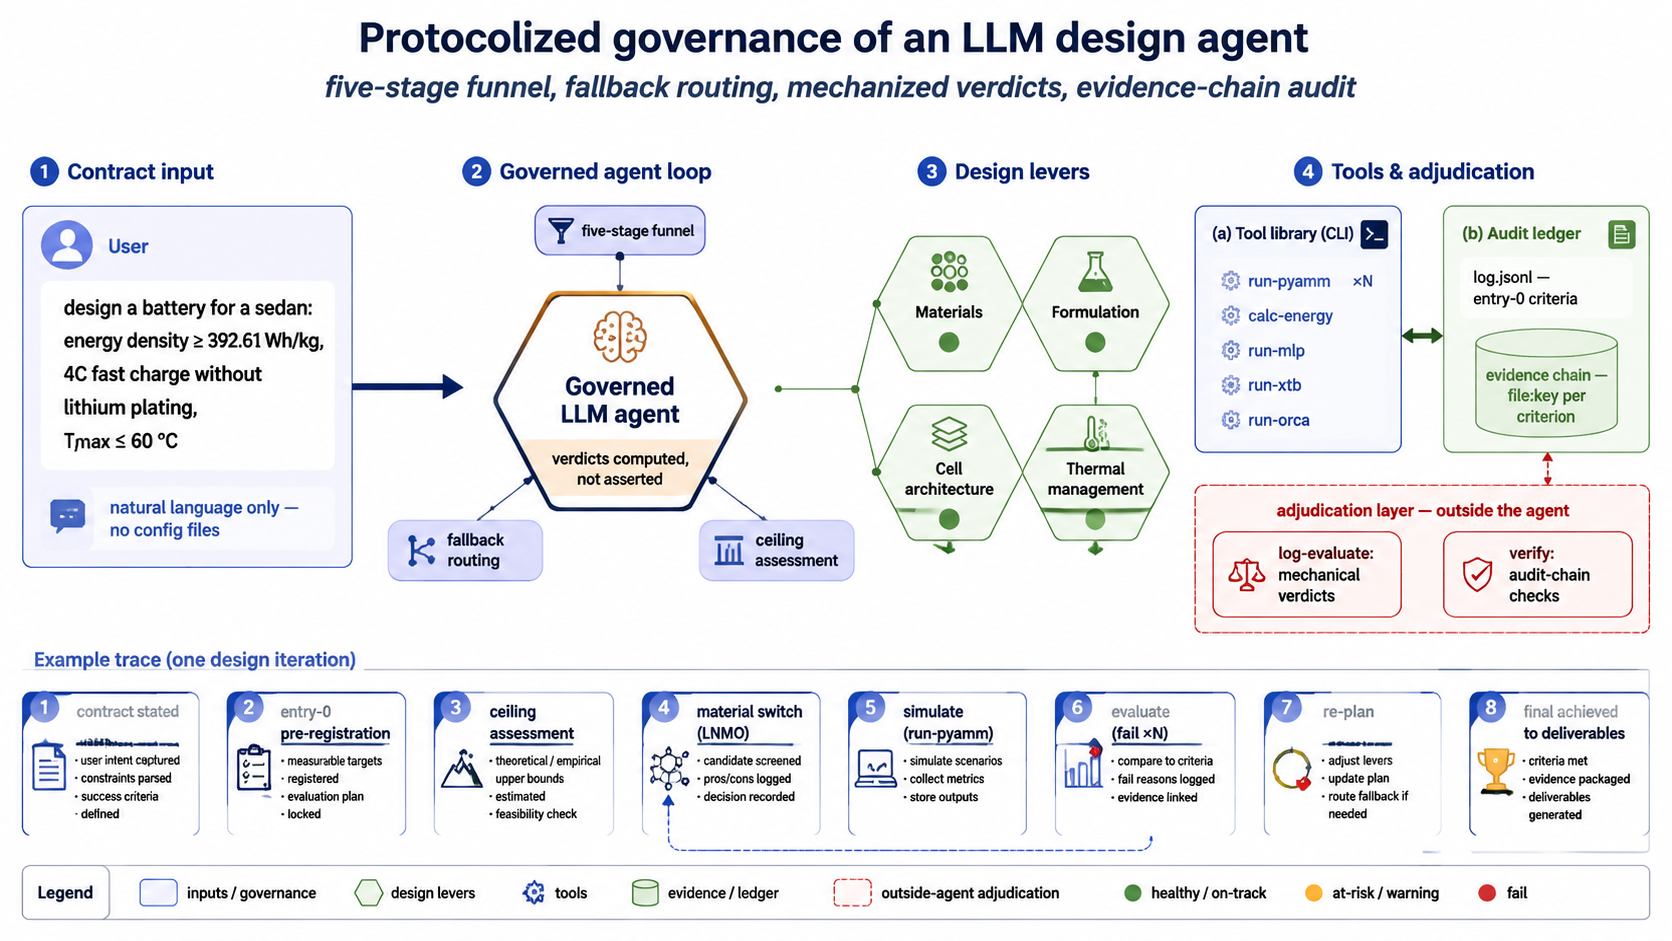
\includegraphics[width=\linewidth]{figs/fig_arch.png}
\caption{System architecture. The natural-language contract is the sole
input; the agent executes the five-stage loop over a command-line tool
library; the adjudication layer sits outside the agent and writes mechanical
verdicts with per-criterion evidence into the audit ledger.}
\label{fig:arch}
\end{figure}

\subsection{The Pipeline and the Five Governance Components}

The protocol organizes work as a five-stage funnel---planning, molecular
screening, cell design, safety assessment, and a closing true-compute
endorsement---inside which five governance components operate as fixed,
always-on rules.

\begin{figure}[!htbp]
\centering
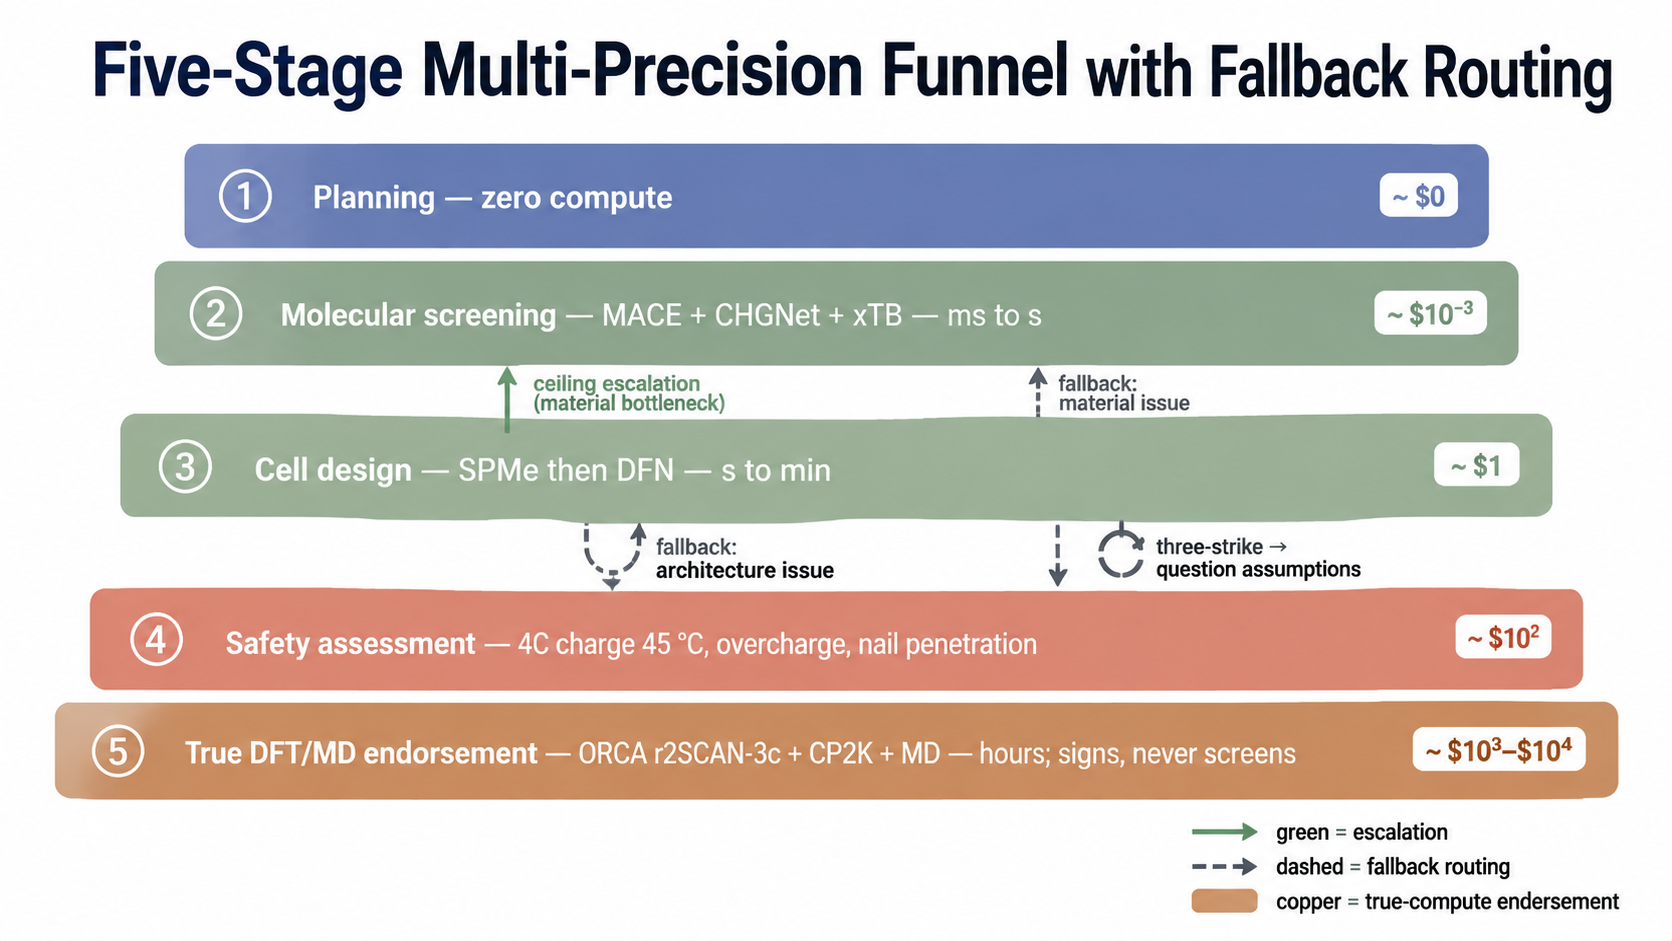
\includegraphics[width=\linewidth]{figs/fig_funnel.png}
\caption{The multi-precision funnel: cost rises from planning (zero
compute) to true DFT/MD endorsement (hours), which signs conclusions and
never screens. Fallback routes a failure to the scale of its cause; ceiling
escalation opens the material lever when the cell-scale ceiling cannot close
the gap.}
\label{fig:funnel}
\end{figure}

\textbf{Component 1: the layered multi-precision funnel with ceiling
escalation.} Screening proceeds from cheapest to dearest: millisecond-scale
machine-learning potentials (MACE \cite{batatia2022mace}, CHGNet
\cite{deng2023chgnet}) and a semi-empirical quantum method (xTB
\cite{bannwarth2019xtb}) at the molecular scale; seconds-scale SPMe then
minutes-scale DFN at the cell scale. The opening of cell design triggers a
\emph{ceiling assessment}: the agent estimates the best architecture-plus-
formulation achievable within the current system and compares it to the
contract. If the objective exceeds the ceiling, the agent is required to
escalate into material design---inventing additives or switching systems---
rather than tuning parameters inside a space that provably cannot close the
gap:
\begin{equation}
\label{eq:escalate}
\text{escalate} \iff \exists c:\; t_c > \mathrm{ceiling}_c(\text{system}),
\end{equation}
where $\mathrm{ceiling}_c(\text{system})$ is the best contract value the
current system's architecture and formulation can reach on criterion $c$. The escalation decision is written to the log with its evidence (which
levers were assessed, the limit values, the gap).

\textbf{Component 2: evaluation and fallback routing.} Every stage output is
evaluated against the contract immediately; on failure, the agent must
diagnose the scale at which the cause lives and fall back there---material
problems to the molecular stage, architecture problems to cell design---not
blindly rerun the pipeline. A three-strike discipline is attached to the
fallback: three consecutive failures with the same cause trigger a
mandatory re-examination of the assumptions (``is this objective physically
reachable in this system?'') rather than a fourth blind attempt. The
symptom-to-scale correspondence is fixed: potential windows and stability
are molecular properties; capacity and temperature rise are architecture
properties.

\textbf{Component 3: heterogeneous model voting.} Every molecular candidate
is screened by three methodologically distinct models---two ML potentials
from different families plus a semi-empirical quantum method---whose
agreement or disagreement is itself signal. Hard elimination lines (energy
above the stability ceiling, non-convergence, HOMO above the oxidation
line) are mechanical; disagreement among the three ranks marks a candidate
\emph{disputed}:
\begin{equation}
\label{eq:disputed}
\text{disputed} \iff \mathrm{spread}(r_1, r_2, r_3) \geq \max(2,\; 0.3 N),
\end{equation}
where $r_1, r_2, r_3$ are the candidate's ranks under the three models
among $N$ candidates---forcing reasoning-based refinement rather than
acceptance or rejection on a single model's word.

\textbf{Component 4: the parameter bridge.} Microscopic properties are
mapped to macroscopic model parameters through a fixed table (Table~\ref
{tab:bridge}); a mistyped parameter name is rejected by the simulator's
validation rather than silently ignored. Every bridge value must carry a
source annotation---literature citation or explicit estimate---and estimates
are prohibited from entering judgment-relevant outputs unlabeled.

\begin{table}[!htbp]
\centering
\caption{The parameter bridge: microscopic property to PyBaMM parameter
names. Mistyped keys are rejected by the simulator (unknown parameter name),
so the table is the safety net against manual transcription error.}
\label{tab:bridge}
\begin{tabular}{ll}
\toprule
Microscopic property & Parameter name (exact key) \\
\midrule
Electrolyte diffusivity & \texttt{Electrolyte diffusivity [m2.s-1]} \\
Electrolyte conductivity & \texttt{Electrolyte conductivity [S.m-1]} \\
Cation transference number & \texttt{Cation transference number} \\
Coating, SEI reaction-limited & \texttt{SEI kinetic rate constant [m.s-1]} \\
Coating, SEI migration-limited & \texttt{SEI reaction exchange current density [A.m-2]} \\
Doping, cracking suppression & \texttt{Positive/Negative electrode cracking rate} \\
\bottomrule
\end{tabular}
\end{table}

\textbf{Component 5: mechanized adjudication and the audit chain.} This is
the load-bearing component. Before the first simulation, the
agent writes entry~0 of the audit ledger: the contract criteria,
pre-registered in machine-readable form and layered by decision stage, with
case-level metadata recording every rule-derived decision and its basis.
Thereafter the agent is \emph{forbidden from judging}: every evaluation must
be issued by the \texttt{log-evaluate} command, which reads the criteria and
the tool-output files, compares each metric against its threshold in code,
and emits a verdict with an evidence chain---for each checked criterion, the
file, the key, the value, and the threshold it was compared against.
A design is ``achieved'' exactly when
\begin{equation}
\label{eq:attain}
\text{achieved} = \bigwedge_{c} \left(v_c \geq t_c^{\min} \;\wedge\; v_c \leq t_c^{\max}\right),
\end{equation}
where the conjunction ranges over the pre-registered criteria of the
contract. Derived criteria are computed mechanically; the plating criterion
is the minimum of the anode potential time series against zero, never a
threshold the agent may pick:
\begin{equation}
\label{eq:plating}
\text{plated} = \left[\min_t \phi_{\text{anode}}(t) < 0\right].
\end{equation}
Equations~\eqref{eq:attain}--\eqref{eq:plating}, like every criterion
expression in this section, are evaluated verbatim by the adjudication
layer. A closing verifier (\texttt{verify-deliverables}) checks the
deliverable set and, crucially, the audit chain itself: every proposal round
must have a same-round mechanical evaluation, and a final judgment entry
must exist---a run whose ledger lacks either is refused as incomplete.
Judgment is thus an infrastructure layer outside the agent, exactly as the
separation of duties in auditing: the auditee may not write its own
verdicts.

The protocol, the tool library, the adjudication layer, and the
cross-harness harnesses are open source
(\url{https://github.com/wangyuanxty/BatteryDesignAgent}).

The fifth pipeline stage is the true-compute endorsement: for the closing
top candidates only, ab initio DFT (ORCA, r2SCAN-3c \cite{neese2022orca})
with optional cross-validation in an independent code (CP2K, PBE-D3
\cite{kuhne2020cp2k}), and molecular dynamics for the top electrolyte
diffusion coefficient. The endorsement \emph{signs} conclusions; it never
screens. In the experiment matrix reported here the endorsement runs are
executed for the flagship cases and reported separately (Section~5.8);
turning it on or off does not change any contract verdict, by design.

\subsection{The Protocol as a Declarative Artifact}

The protocol is packaged as a self-contained declarative artifact: a
natural-language rule set, a command-line tool library (twenty-plus
simulation, evaluation, and audit commands), and the audit ledger format.
It binds to no agent framework---any harness that can loop a model over a
shell and files can execute it. The governance travels with the contract,
not with the harness. In the present study every run executes under one
harness; cross-harness portability is a structural property by
construction, and its empirical demonstration (the same protocol under
additional agent frameworks) is demonstrated empirically with identical contract outcomes (Section~5.7).

\subsection{Implementation}

The tool library is implemented as a Python package over PyBaMM
\cite{sulzer2021pybamm} for electrochemistry---including the
thermal-electrochemical parameters \cite{oregan2022electrochim} and
degradation physics \cite{okane2022pccp, peled1979sei,
arora1999plating, ren2018plating, wang2012thermalrunaway}---plus surrogate
and true-compute runners. Twenty-plus commands cover simulation protocols
(discharge at 1C/0.1C/5C, 4C charge at 45\,$^\circ$C, low-temperature
discharge, overcharge, 100-cycle aging, nail penetration with a
three-reaction thermal-runaway ODE), contract-caliber energy accounting, the
mechanical evaluator, and the deliverable verifier. The adjudication layer
is pinned by an automated regression suite distributed with the tool
library.
All conclusion-grade numbers in every report originate in tool outputs;
the ledger is the paper's primary data source, and every figure and table
here is derivable from it.

% ============================================================
% 4. Experimental Design
% ============================================================
\section{Experimental Design}
\label{sec:experiments}

\subsection{Task Suite}

The task suite consists of eight scenario tasks, each a natural-language
requirement written as an application scenario plus absolute numeric
criteria (Table~\ref{tab:tasks}). The scenarios span the design landscape
deliberately: a sedan (performance plus thermal safety), grid storage
(cycle life plus low temperature), power tools (rate plus power), extreme
cold (low temperature plus volumetric density), a flagship vehicle (extreme
energy density), a smartphone (volumetric ceiling plus a strict temperature
red line plus a voltage plateau), a hybrid vehicle (high-temperature aging
plus nail penetration), and a drone (specific energy plus a mass ceiling).
Across the eight tasks, fourteen distinct metric types are checked, and
all criteria of a task are AND-judged: a design must satisfy every clause
of its target to be ``achieved.''

Three design choices deserve emphasis. First, the tasks carry no constraint
declarations beyond the metrics: nothing states which variables are adjustable,
which chemistry to use, or where the baseline sits. Undeclared items are
interpreted in the widest sense under the workflow rules, with the derivation
recorded---this is what forces the agent to make the design-space decisions
itself. Second, every number in every task is absolute; no relative-baseline
phrasing appears, so an agent cannot redefine the reference it measures
against. Third, the tasks are heterogeneous in where their binding
constraint lives: T1, T4, and T8 are solvable inside a structural space
(thickness, porosity, mass), while T2, T3, T5, T6, and T7 require material,
formulation, or transport variables---the distinction on which the comparison
with the Bayesian baseline turns.

The target quantities are defined on standard cell models from the cited
literature. Plating is judged on the negative-electrode potential against
Li/Li$^+$, written as the sum of the equilibrium potential and the kinetic
overpotential \cite{arora1999plating, ren2018plating}:
\begin{equation}
\label{eq:phi}
\phi_{a} = U_a + \eta_c.
\end{equation}
The SEI criterion reads a state variable of the degradation model, whose
growth law supplies the coating variable that T2 and T6 exploit
\cite{peled1979sei, okane2022pccp}:
\begin{equation}
\label{eq:sei}
\frac{d\delta}{dt} = k_{\mathrm{SEI}},
\end{equation}
where $k_{\mathrm{SEI}}$ is exactly the parameter the electrode-modification
bridge adjusts. The thermal-runaway trigger for the overcharge and
nail-penetration criteria is the three-side-reaction energy balance
\cite{wang2012thermalrunaway}:
\begin{equation}
\label{eq:tr}
m c_p \frac{dT}{dt} = \sum_k \Delta H_k r_k(T) - hA\,(T - T_{\mathrm{amb}}),
\end{equation}
with $\text{triggered}$ iff the trajectory crosses the runaway onset; the
cooling coefficient $h$ is the thermal-management variable. Criterion values are model-relative (an SEI limit reads the state variable
of a specific degradation model, a plateau reads a specific OCP set) so
cross-system comparisons are made only within the same model. The scenario
anchoring (which production
specification each task draws from, and how each threshold was calibrated
from the underlying parameter sets) is documented in the supplementary
materials; each threshold is the anchoring parameter set's baseline value
for that criterion shifted by a fixed increment (e.g., $+20\%$ energy
density over the baseline configuration, a $5$-point cut on 5C retention),
never a frontier-tight value---the experiment measures the workflow's
contribution at fixed targets, not frontier performance. The anchoring is
a Methods-section explanation and never appears in the task text seen by
any agent.

\begin{table}[!ht]
\centering
\caption{The eight scenario tasks. Every criterion is an absolute number,
AND-judged; nothing else is declared in the task text.}
\label{tab:tasks}
\setlength{\tabcolsep}{2.5pt}
\begin{tabular}{p{1.0cm}p{10.5cm}}
\toprule
ID & Design target (abridged; all values absolute) \\
\midrule
T1 & Sedan: energy density $\geq 392.61$ Wh/kg; 4C charge without lithium
plating; $T_{\max}\leq 60\,^\circ$C; overcharge to 4.7 V without thermal
runaway. \\
T2 & Grid storage: energy density $\geq 327.18$ Wh/kg; 4C charge without
plating; SEI $\leq 500$ nm after 100 cycles; $\geq 90\%$ capacity retention
at $-20\,^\circ$C; SEI $\leq 550$ nm after 500 cycles. \\
T3 & Power tools: capacity $\geq 2$ Ah; 5C retention $\geq 95\%$; 4C charge
without plating; $T_{\max}\leq 60\,^\circ$C; power density $\geq 4000$
W/kg. \\
T4 & Extreme cold: $\geq 95\%$ 1C retention at $-20\,^\circ$C; energy
density $\geq 327.18$ Wh/kg; volumetric energy density $\geq 880$ Wh/L. \\
T5 & Flagship: energy density $\geq 500.94$ Wh/kg; 4C charge without
plating; $T_{\max}\leq 60\,^\circ$C. \\
T6 & Smartphone: volumetric energy density $\geq 950$ Wh/L; 4C charge
without plating; $T_{\max}\leq 50\,^\circ$C; SEI $\leq 500$ nm after 100
cycles; voltage plateau $\geq 4.1$ V. \\
T7 & Hybrid: energy density $\geq 327.18$ Wh/kg; 4C charge without plating;
SEI $\leq 550$ nm after 100 cycles at $45\,^\circ$C; nail penetration
(10 W short-circuit heat) without thermal runaway. \\
T8 & Drone: energy density $\geq 446.18$ Wh/kg; 5C retention $\geq 90\%$;
cell mass $\leq 40$ g. \\
\bottomrule
\end{tabular}
\end{table}

\subsection{Conditions and Control Groups}

The design follows a treatment-plus-two-controls structure. The governed
agent is the treatment; two control groups isolate, respectively, the
workflow itself and the classical-optimization boundary. All three
conditions share the task texts, the simulation stack, and the session
budget, so each observed difference is attributable to the single variable
that condition removes.

\textbf{Governed agent (G).} The full workflow of Section~3, executed under
two large language models separately (deepseek-v4-pro and
deepseek-v4-flash) giving eight runs per model and a model-robustness
axis. Two further runs re-execute the eight sessions under GPT-5.6 Luna
and under mimo-v2.5 (two other models served through
OpenAI-compatible APIs, same workflow, harness, task texts, and budget) so
the cross-family comparison is made on models outside the primary family at matched
tier logic.

\textbf{The design workflow-free agent (C1).} The same LLM, the same agent harness
(tool-use loop), the same session budget, and the same task texts---but the
workflow is removed in full: both its written layer (stage rules, the funnel,
criteria, the evaluator, the audit-chain verifier) and its
instrument, the curated simulation library that ships inside the workflow's
skill directory and encodes the workflow's calibration choices (its named aging
workflow, its energy-density caliber, its screening recipes). The control
retains the general-purpose simulation stack---a Python interpreter with PyBaMM,
MACE, CHGNet, ASE, pymatgen and RDKit, plus shell and file tools---and, in the
current design, its prompt states the interpreter path and the installed
libraries with their entry points, recording explicitly that no workflow,
workflow, or measurement standard is prescribed. What the condition removes is
therefore not capability but \emph{pre-committed measurement machinery}: to
obtain an aging result, an energy density, or a screening verdict, the
workflow-free agent must construct the chain itself and choose its own
definitions. One run per task, deepseek-v4-pro. The batch tabulated in
Section~5.5 was run with the general-purpose libraries only (no curated
tooling) and without an environment statement in its prompt; that asymmetry is
disclosed there, its claims are re-checked against the given targets, and
the batch is therefore reported as a bundled condition rather than as an
equal-tooling control.

\textbf{Bayesian optimization (C2).} A classical BO baseline in the
architecture parameter space (ten structural parameters: electrode
thicknesses and porosities, separator thickness and porosity, current
collector thicknesses, heat transfer coefficient, negative particle radius),
searching the objective \emph{energy density minus safety penalties},
\begin{equation}
\label{eq:bo}
\mathrm{obj} = \mathrm{ED} - \sum_{k} \lambda_k\, \mathbb{1}[v_k \not\geq t_k],
\end{equation}
with a fixed penalty set that covers every target criterion except the
T1 overcharge-runaway trigger (plating, temperature limit, SEI, plateau,
mass); a criterion absent from this set is invisible to the search. The
material-bottleneck failures are therefore not a visibility artifact: SEI
and plateau \emph{are} penalized (a re-run with the aligned $50\,^\circ$C
red line confirms the failures persist, Section~5.1). What the optimizer
cannot do is move a chemistry switch, because its knob space is
structural only---and that boundary is the point: the configuration
replicates Battery-Sim-Agent's published BO standard
\cite{chen2026battery}: Meta's Ax platform, Sobol initialization, GPEI with
LogNEI acquisition, fixed seed 1234, fifty evaluations per task---the same
simulator and the same prescribed energy accounting as the agents, so
the comparison is on identical physics. The search is deterministic in its
seed; a three-seed replication (1234, 5678, 9012) reproduces the attained-task
set $\{T1,T4,T8\}$ identically, with per-task best objectives within $9\%$
across seeds (supplementary materials). C2 is the \emph{classical-baseline
control}: it isolates the solution-space boundary of ungoverned search: a
strong, published-standard optimizer that cannot leave its parameter space.
One run (fifty evaluations) per task.

\textbf{Resources held constant.} All three conditions receive the same
task texts, the same simulation stack, and the same session budget: the
agents run under the same harness turn budget (the agent SDK's
\texttt{max\_turns}=300 setting) and the workflow carries no round cap of
its own. Under the SDK's turn definition---one user-message
$\leftrightarrow$ assistant-response pair---the extension run T10, the
longest governed session, consumed 207 turn pairs (303 assistant
messages); the longest control session hit the cap at 443. Table~4
reports a log-derived activity metric, \emph{assistant messages}, the
finer-grain counterpart of the SDK turn counter; the budget
\emph{setting}, not the message count, is the controlled resource. The
BO baseline's fifty evaluations define its budget. A second, simulator-native currency is likewise anchored: the
governed sessions average 25 run-pyamm calls per task (range 0--55; 31
including calc-energy), against BO's fixed fifty: the agents hold no
evaluation-count advantage, and both conditions sit in the same order of
magnitude on every resource axis. Neither currency is equalized per
operation; each condition receives its method family's standard budget, and
the comparison is made at that level. True-compute endorsement is disabled
across the main matrix
($\texttt{real\_compute}=\texttt{false}$); endorsement results are reported
separately in Section~5.8.

\subsection{Ablation Design}

These rules are fixed properties of the workflow; ablation is
an experimental intervention that relaxes exactly one rule per run.
An ablation variant is declared in the task text itself (``ceiling
escalation disabled'') (keeping the natural-language requirement the sole
entry point) and the declaration is recorded in the run's entry-0 metadata.
Three ablations are executed: \emph{ceiling escalation off} (no proactive
material-design escalation; the agent tunes within the current system unless
the text names materials), on T2/T5/T6; \emph{architecture forcing off} (no
required 2--4 architecture variants per round), on T1/T2/T3/T4/T7/T8; and
\emph{funnel voting off} (molecular screening by a single ML potential
instead of three-model heterogeneous voting), on T2/T5/T6. Each ablation run
uses deepseek-v4-pro and the full workflow otherwise. Twelve ablation runs
in total.

\subsection{How Designs Are Evaluated}

All verdicts reported in this paper come from the code-based evaluation
layer of Section~3: criteria pre-registered in entry 0, verdicts computed
by \texttt{log-evaluate} from tool-output files, evidence chains per
criterion, and the deliverable verifier's audit-chain checks. Two further
audits are applied to the control conditions. For C1, the agent's own
``achieved'' claims are re-checked at the workflow's target caliber by
the authors: every claimed metric is recomputed by code from the
artifact files the agent produced, on the workflow's own definitions. Two calibers recur throughout and are fixed here:
\begin{equation}
\label{eq:ed}
\mathrm{ED} = \frac{\int V(t)\, I\, dt}{\sum_i l_i\,(1-\varepsilon_i)\,\rho_i \cdot A},
\end{equation}
the prescribed energy density (mass = layer stack, electrolyte
excluded), and
\begin{equation}
\label{eq:ret}
\mathrm{ret}_{5C} = C_{5C}/C_{1C},
\end{equation}
the rate-retention caliber against the 1C reference. The power criterion is
computed from the discharge-start voltage drop and the cell mass (standard
definitions of DC resistance and peak power):
\begin{equation}
\label{eq:power}
\mathrm{DCR} = \frac{V(0) - V(t_{10\%})}{I},
\qquad
P_{\max} = \frac{V_{\mathrm{oc}}^2}{4\,\mathrm{DCR}\cdot m},
\end{equation}
with $V(t_{10\%})$ the voltage at 10\% of discharge time. A claim computed
against a different reference (e.g., 5C over C/3) or a different mass model
is a different caliber and is recomputed (nail penetration means a
thermal-runaway trigger criterion, not a steady-state temperature). For C2, the objective trajectory
is recomputed from the logged evaluation outputs. The re-checking rules
are applied by code and are listed in the supplementary materials.

\subsection{Real-Data Anchor}

To anchor the simulation world to a physical artifact, the calibrated
parameter set for the LG M50 cell \cite{oregan2022electrochim} is compared
against the beginning-of-life $0.1$C discharge of a production LG M50T
21700 cell from the Imperial College degradation dataset
\cite{lgm50dataset2024, kirkaldy2024lgm50}: measured capacity 4878.9 mAh
versus simulated 4857.0 mAh ($+0.45\%$), and voltage-curve RMSE 20.6 mV
over 2--82\% depth of discharge. The alignment is the Methods-section
calibration record; it establishes that the numbers agents are judged
against are anchored to a production cell: a validation of the simulator,
not of the final designs (Section~6). Figure~\ref{fig:alignment} overlays
the measured and simulated curves.

\begin{figure}[!ht]
\centering
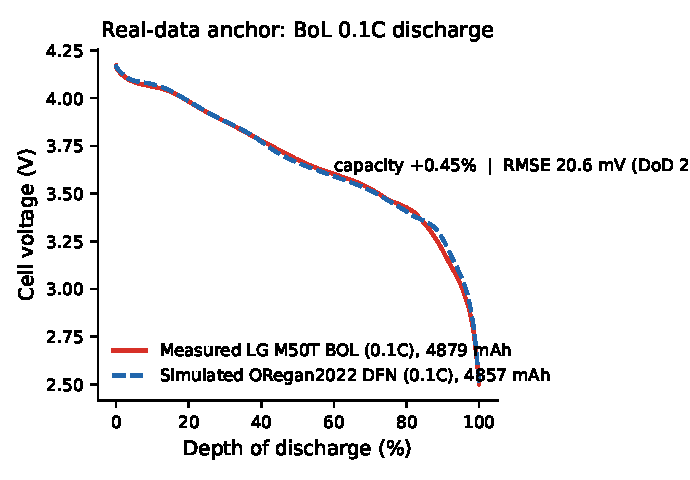
\includegraphics[width=0.78\linewidth]{figs/fig_alignment.pdf}
\caption{Real-data anchor: beginning-of-life $0.1$C discharge of a
production LG M50T 21700 cell (Imperial College dataset,
\cite{lgm50dataset2024}) versus the ORegan2022-parameterized DFN simulation
\cite{oregan2022electrochim}. Capacity agrees to $+0.45\%$; voltage RMSE
$20.6$ mV over 2--82\% depth of discharge.}
\label{fig:alignment}
\end{figure}

\subsection{Cross-Harness Portability}

The workflow's independence from any specific agent framework
(Section~3.4) is a design property of the artifact itself; its empirical
demonstration is reported here and executed in Section~5.7, so that its
results slot into Section~5 without methodological ambiguity. The design:
the identical workflow (the same declarative rule set, the same
command-line tool library, and therefore the same evaluator) runs
the same task texts (T1, a structural-bottleneck target, and T6, a
material-bottleneck target) under the same LLM and the same nominal budget setting
(300, in each harness's own turn unit) across three harnesses: the harness used throughout this paper, the
OpenAI Agents SDK, and LangChain. The measured quantities are target
attainment (checked by code, identical criteria) and audit-chain
completeness (the verifier's checks). Because the evaluator is a
command-line tool rather than harness code, the verdict mechanics are
harness-independent by design; the experiment measures whether agent
behavior under the same workflow remains faithful to the given targets when the
orchestration substrate changes, as reported in Section~5.7.

% ============================================================
% 5. Results
% ============================================================
\section{Results}
\label{sec:results}

\subsection{Main Comparison: Target Attainment}

Table~\ref{tab:main} reports target attainment for all eight tasks under
the six columns. Three findings stand out. First, the governed
agent achieves \textbf{8/8} under the two primary models and \textbf{4/8}
under each of the two other models (Section~5.4); every verdict is
computed in code, with an evidence chain per criterion and a verifier-passed
audit chain. Second,
the Bayesian optimizer achieves \textbf{3/8}: exactly T1, T4, and T8, the
three tasks whose binding constraint is structural (thickness, porosity,
mass). Its best designs reach energy densities above the governed agent's on
these tasks (e.g., 678 versus 472 Wh/kg on T4), the expected consequence of
an unconstrained thin-electrode search against a margin-balanced design; on
the remaining five tasks it fails on the design target's own criteria: 4C
plating in T2, T3, T5, T6, T7; SEI limits in T2, T6, T7; a catastrophic
$3.44\%$ 5C retention on T3; the 4.1 V plateau unreachable on T6, where
the best design stalls at the NMC811 plateau limit ($4.0065$ V)---a re-run
with the penalizer aligned to the design target's $50\,^\circ$C red line (the
main run hardcoded $60\,^\circ$C) leaves the outcome unchanged: 0/50 trials
attain the design target in either configuration, 30/50 clear the volumetric
criterion alone in the aligned run, and none is simultaneously
plating-free and below the red line; nail penetration triggered on T7. Figure~\ref{fig:bo} shows the BO trajectories: the three structural
tasks climb to attainment, the five material-bottleneck tasks plateau
against penalties no structural parameter can remove. Third, in the tabulated
workflow-free batch---whose tool asymmetry is disclosed in Section~5.5---no
claim survives within the
measurement space: two of its claimed successes (T4, T8) solve the design target
by switching to a lithium-metal cell outside the validated parameter sets,
and its remaining claims fail re-checking against the criteria (Section~5.5). The
tie between the two baselines (three achieved tasks each) with orthogonal
failure modes is the paper's central observation: the bare agent and the
black-box optimizer fail for different, specifiable reasons, and only the
governed agent passes on all eight targets.

Target-margin calibration deserves explicit reporting, since ``8/8''
could otherwise read as loose thresholds. The thresholds are fixed
increments over the anchoring parameter sets' baseline values, not
frontier-tight values (Section~4.1), and all three conditions face
identical targets: any looseness benefits the baselines equally. The
achieved margins show the design targets binding where they are meant to bind:
on six of the eight governed runs the last criterion to clear sits within
$4.5\%$ of its threshold (T6's plateau at $+0.4\%$ and thermal line at
$+0.5\%$; T8's mass at $+0.5\%$; T3's and T5's thermal lines at
$+1.0$--$1.5\%$); the two exceptions are T2's low-temperature retention
($+10.6\%$) and T7's SEI limit ($+15.4\%$). The wide margins concentrate
on the energy-density clauses of the structural tasks ($+41$--$48\%$),
where an unconstrained thin-electrode search overshoots cheaply; the same
mechanism behind the BO's 678 versus 472 Wh/kg on T4, and precisely the
margin the governed designs partially spend on the safety and durability
criteria. Per-criterion margins for all achieved runs are tabulated in the
supplementary materials. The SEI criteria deserve one further disclosure,
because they are the single criterion class whose bridge lever (the
electrode-modification coating scaling the SEI kinetic rate constant) can
move a verdict: T2 shipped a $10^{-4}\times$ rate constant (declared in
the audit as an estimate beyond the bare-ALD literature magnitude), yet the
identical design passes the design target at $10^{-2}\times$ (500.4 nm against
the 550 nm limit, a $9\%$ margin); T6's SEI work is not verdict-bearing;
T7 used no kinetic override (supplementary materials).

The thresholds are author-anchored, and one threshold property should be
stated in advance of the reader's own check: the comparison's direction is
invariant under a uniform perturbation of them. On the five
material-bottleneck tasks the optimizer's failure is ceiling-bound, not
threshold-bound---across all 400 baseline trials, the highest midpoint
voltage any design reaches is 4.0115 V against the 4.1 V target line, and
plating and SEI violations are lever-bound (supplementary materials). On the
three structural tasks the same criteria bind both conditions in parallel:
under a uniform $+5\%$ tightening the optimizer's attained counts fall from
25/34/10 to 0/22/1, while the governed runs' own binding margins
($+2.2\%$/$+4.5\%$/$+0.5\%$ on T1/T4/T8, Appendix~B of the
supplementary materials) fail
under the same tightening on the same tolerance. No $\pm 5\%$ perturbation
inverts the direction of the comparison; the only conceivable inversion
zone---energy-density thresholds above the governed designs' own margins,
$>+40\%$ on the structural tasks---is exactly the region in which the paper
already reports the optimizer's structural-task energy-density superiority.

\begin{figure}[!ht]
\centering
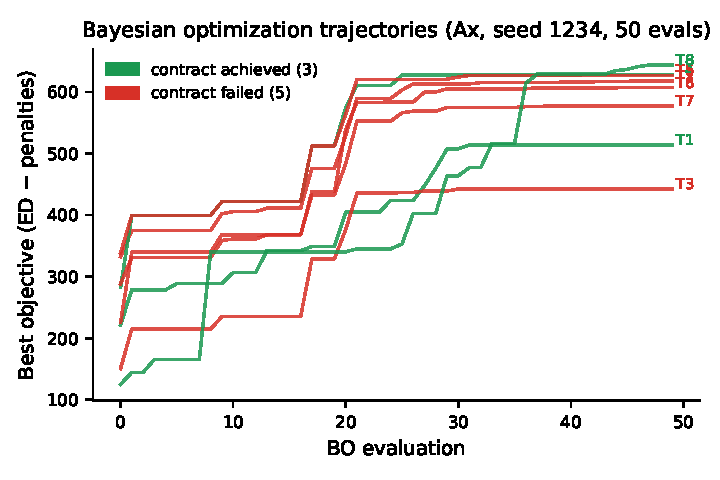
\includegraphics[width=0.8\linewidth]{figs/fig_bo_trajectories.pdf}
\caption{Bayesian optimization best-objective trajectories per task (Ax,
Sobol initialization, GPEI + LogNEI, seed 1234, 50 evaluations). The three
structural tasks (T1/T4/T8) achieve their targets; the five
material-bottleneck tasks plateau against penalties (plating, SEI, plateau,
nail) that no structural parameter can remove.}
\label{fig:bo}
\end{figure}

\begin{table}[!ht]
\centering
\footnotesize
\setlength{\tabcolsep}{3.2pt}
\caption{Target attainment, eight tasks $\times$ six columns
(governed agent shown under four models: pro, flash, luna, mimo).
$\checkmark$ = achieved (code-computed verdict); $\times$ = failed target
criteria; $\circ$ = outside the measurement space (see text). G = governed
agent; C1 = workflow-free agent; C2 = Bayesian optimization. Key re-checked
numbers in parentheses. Per-task numbers are r1 values; the condition
totals are seed-robust as detailed in the table note and supplementary
materials.}
\label{tab:main}
\setlength{\tabcolsep}{1.6pt}
\begin{tabular}{p{0.125\linewidth} p{0.135\linewidth} p{0.135\linewidth} p{0.135\linewidth} p{0.135\linewidth} p{0.135\linewidth} p{0.135\linewidth}}
\toprule
Task & G (pro) & G (flash) & G (luna) & G (mimo) & C1 & C2 \\
\midrule
T1 sedan & $\checkmark$ 553.98 & $\checkmark$ 459.4 & $\times$ (plating) & $\times$ (plating) & $\times$ ($-6.9$ mV) & $\checkmark$ 514.13 \\
T2 storage & $\checkmark$ 465.62 & $\checkmark$ & $\checkmark$ & $\checkmark$ & $\times$ (plating, SEI) & $\times$ (plating, SEI) \\
T3 tools & $\checkmark$ & $\checkmark$ & $\checkmark$ & $\checkmark$ & $\times$ (5C 84.8\%) & $\times$ (plating, 5C) \\
T4 cold & $\checkmark$ 471.55 & $\checkmark$ & $\checkmark$ & $\times$ (plating) & $\circ$ (Li-metal) & $\checkmark$ 678.26 \\
T5 flagship & $\checkmark$ & $\checkmark$ & $\times$ (ceiling) & $\checkmark$ 517.8 & $\times$ ($-12.6$ mV) & $\times$ (plating) \\
T6 phone & $\checkmark$ 1135.8 & $\checkmark$ & $\times$ (895.6 Wh/L) & $\times$ (852.8 Wh/L) & $\times$ budget & $\times$ (plateau, $T_{\max}$) \\
T7 hybrid & $\checkmark$ & $\checkmark$ & $\checkmark$ & $\checkmark$ & $\times$ (nail unproven) & $\times$ (plating, nail) \\
T8 drone & $\checkmark$ & $\checkmark$ & $\times$ (mass) & $\times$ (mass, $T_{\max}$) & $\circ$ (Li-metal) & $\checkmark$ 643.75 \\
\midrule
\textbf{Total} & \textbf{8/8} & \textbf{8/8} & \textbf{4/8} & \textbf{4/8} & \textbf{0/8 in-space} & \textbf{3/8} \\
\bottomrule
\end{tabular}
\par\vspace{3pt}
\footnotesize
G (pro): three-seed replication (r1--r3); every attained task achieved
in all three seeds ($24/24$, supplementary materials). G (flash), G (luna),
G (mimo), and C1: one run per cell, as stated in the respective sections.
C2: three seeds (1234/5678/9012); attained set $\{T1,T4,T8\}$ in all three.
The mimo T1 run omitted the final ledger entry; under the audit-chain rule it
is counted as not attained (Section~5.4).
\end{table}

\subsection{Resource Cost}

Table~\ref{tab:cost} reports the governed agent's resource consumption per
task under both models: assistant messages (activity measure) and model
tokens (input/output) and Figure~\ref{fig:cost} plots the same data,
highlighting the material-bottleneck peaks (T6 and, under flash, T5).
Three observations. Material-bottleneck tasks are the expensive ones: T6
(the smartphone target demanding a cathode-system switch) consumes 468
messages and the largest token counts under pro, and T5/T6 dominate under
flash. The economy model completes the suite at roughly three-quarters of
the flagship model's input tokens (1.12M versus 1.52M) and 2,418 versus
2,723 assistant messages, with zero attainment difference: the workflow, not the model,
absorbs the difficulty. The C1 runs run under the same harness budget
setting per task (one, T6, hit it); the BO baseline consumes fifty simulator evaluations per task (400 in
total).

\begin{figure}[!ht]
\centering
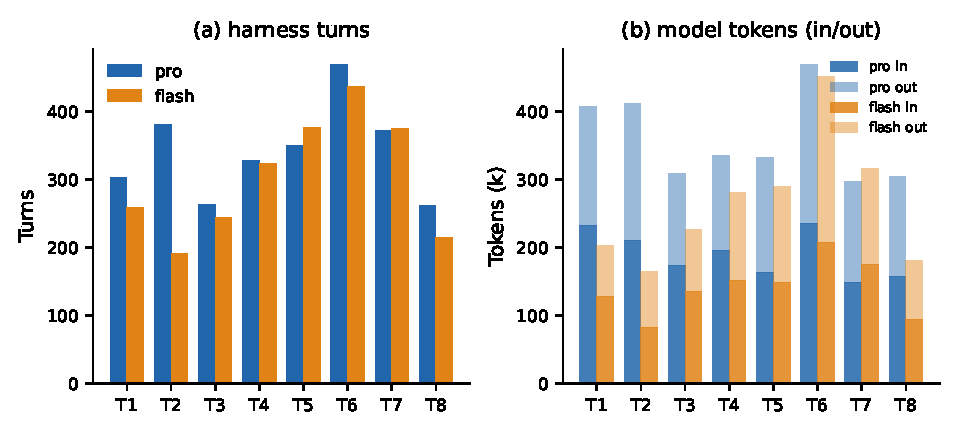
\includegraphics[width=\linewidth]{figs/fig_cost.pdf}
\caption{Governed-agent resource cost per task under both models: (a)
assistant messages; (b) model tokens in/out (thousands). Material-bottleneck
tasks (T6, and T5 under flash) are the expensive ones; the economy model
completes the suite at 8/8 with roughly three-quarters of the flagship
model's input tokens.}
\label{fig:cost}
\end{figure}

\begin{table}[!ht]
\centering
\caption{Governed-agent activity per task (assistant messages; tokens in/out in
thousands). Assistant messages are a log-derived activity measure; the
controlled budget is the identical harness setting across all sessions.}
\label{tab:cost}
\begin{tabular}{lccccc}
\toprule
 & \multicolumn{2}{c}{pro} & \multicolumn{2}{c}{flash} \\
\cmidrule(lr){2-3}\cmidrule(lr){4-5}
Task & msg. & tok. in/out & msg. & tok. in/out \\
\midrule
T1 & 303 & 232/176 & 258 & 128/75 \\
T2 & 380 & 210/202 & 191 & 82/83 \\
T3 & 263 & 173/136 & 244 & 136/91 \\
T4 & 327 & 196/139 & 323 & 152/129 \\
T5 & 350 & 164/169 & 376 & 149/141 \\
T6 & 468 & 235/234 & 437 & 207/245 \\
T7 & 371 & 149/148 & 374 & 175/142 \\
T8 & 261 & 158/147 & 215 & 94/87 \\
\midrule
Total & 2723 & 1517/1352 & 2418 & 1123/992 \\
\bottomrule
\end{tabular}
\end{table}

\subsection{Ablation: Which Components Carry the Effect}

Table~\ref{tab:ablation} reports the twelve ablation runs, and
Figure~\ref{fig:ablation} summarizes their verdicts as a per-component
stacked bar. The three mechanisms contribute at very different magnitudes,
and the decomposition is the paper's answer to RQ2. Ceiling escalation is the load-bearing
mechanism: disabling it costs two of the three material-bottleneck tasks
outright: T6 loses its LNMO system switch (the 4.1 V plateau is unreachable
in NMC811 space) and T2 loses its SEI-kinetics bridge (three of five
criteria pass, the in-space result): while T5, whose tipping point
turned out to live inside the configuration space, is unaffected.
Architecture forcing is a narrow lever: disabling it changes exactly one
task (T2), where forced breadth was the exploration that found the design.
Funnel voting shows no verdict change in any of its three cells: with the three-model vote off,
the molecular path was actually taken \emph{more} often (six molecules
screened on T2, three on T6, versus none in the baseline runs), and the
single-model screenings still led to achieved targets. In this task suite the
voting mechanism showed no verdict change in any cell: one run per cell,
so the null is an observed absence rather than a statistical claim; it is
consistent with the mechanism's role as defensive instrumentation that the
baseline never exercised, and with Battery-Sim-Agent's
reported low-headroom calibration \cite{chen2026battery}. The
material-innovation axis stayed dormant throughout: every bottleneck in the
suite closed on the cheaper routes (system switches, electrode-modification
bridges, formulation matching, known candidates; Section~3.1), so the
workflow's free-generation and composition-search freedoms were never
needed.

\begin{figure}[!ht]
\centering
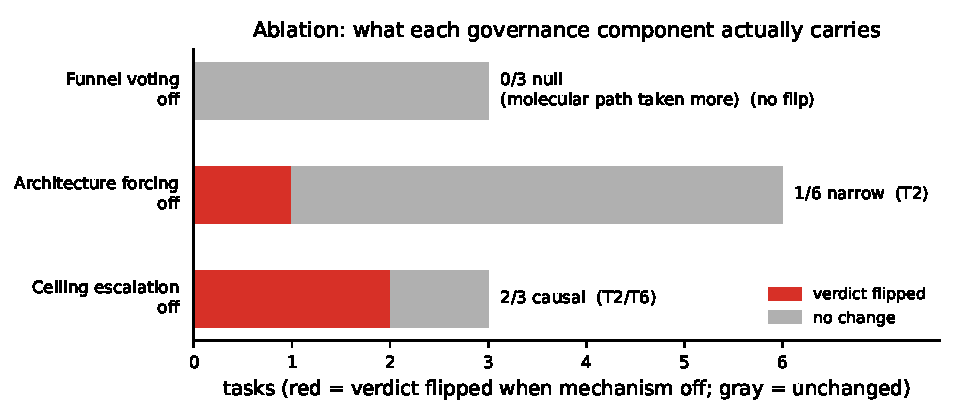
\includegraphics[width=\linewidth]{figs/fig_ablation.pdf}
\caption{What each workflow rule actually carries: red segments count
the tasks whose verdict flipped when the rule was disabled; gray
segments count the unchanged tasks. Ceiling escalation is causal for two of
three material-bottleneck tasks; architecture forcing for one of six;
funnel voting for none: no verdict change observed in this suite.}
\label{fig:ablation}
\end{figure}

\begin{table}[!ht]
\centering
\caption{Ablation results: verdict with the component disabled versus the
full-workflow verdict (F). $\checkmark$ = achieved; $\times$ = not
achieved. The T5 voting-off cell is a no-op: the molecular funnel was not
exercised in that task (start stage = cell design), so the cell carries no
inference about the voting mechanism.}
\label{tab:ablation}
\begin{tabular}{lcccc}
\toprule
Task & ceiling off & force off & voting off & full workflow \\
\midrule
T1 & -- & $\checkmark$ & -- & $\checkmark$ \\
T2 & $\times$ (3/5) & $\times$ & $\checkmark$ & $\checkmark$ \\
T3 & -- & $\checkmark$ & -- & $\checkmark$ \\
T4 & -- & $\checkmark$ & -- & $\checkmark$ \\
T5 & $\checkmark$ & -- & $\checkmark$ & $\checkmark$ \\
T6 & $\times$ & -- & $\checkmark$ & $\checkmark$ \\
T7 & -- & $\checkmark$ & -- & $\checkmark$ \\
T8 & -- & $\checkmark$ & -- & $\checkmark$ \\
\bottomrule
\end{tabular}
\end{table}

\subsection{Model Robustness}

The workflow is model-robust: 8/8 under the two DeepSeek models, with the same
targets attained through different designs---and under the pro model the
8/8 is not an artifact of a single run: all eight tasks were repeated under
three seeds, and every attained task achieved in all three
($24/24$, supplementary materials). On T5 the pro run settled on a
dual-validated architecture design while the flash run took the
material-funnel route (LNMO, with FEC/VC/PES/DTD passing the funnel); on T1
the designs differ by 94 Wh/kg in opposite-margin strategies yet both meet
every criterion. Target attainment is reproducible across models; the
solution space remains broad. One execution defect surfaced and was absorbed by the audit layer: the
flash T6 run delivered a verifier-passed deliverable set but omitted the
final judgment entry from its ledger; the mimo T1 run repeated the same
omission. The verifier now refuses such incomplete audit chains and counts
the run as not attained: the defect became a regression test, which is
precisely the purpose of the audit infrastructure.

Two further runs extend the robustness question across model families:
the same eight sessions re-executed under GPT-5.6 Luna and under
mimo-v2.5 (two other models served through OpenAI-compatible
APIs) with the same workflow, harness, task texts, and budget. Both runs
attain $4/8$ (Luna on T2, T3, T4, T7 and mimo on T2, T3, T5, T7) and
their non-attainments differ revealingly from the baselines'. First, both
are honest: Luna's four are code-computed \emph{not-achieved} verdicts with
complete evidence chains, and mimo reports its failing criteria in the
recommendation itself (T8 is self-labeled ``achieved with documented
limitations'' because mass and thermal fall outside the design target; T6 is a
code-computed not-achieved). Second, the intersection $\{T2, T3, T7\}$ is
attained under every one of the four models (the stability point of the
claim about the workflow) while the disagreements are model-specific and
informative: T4's plating line survived Luna's design but not mimo's, whose
final design report concedes the plating clause even as its ledger carries
``achieved'' (an overdeclaration the audit records as such); on T5, mimo
found the thin-electrode plus high-transport-electrolyte route that eluded
Luna. Third, the joint non-attainments concentrate exactly where the
governed DeepSeek runs needed the ceiling-escalation mechanism: T1 falls to
plating under both other models, T6 stalls at the NMC811 plateau
(mimo: 852.8 Wh/L and 3.97 V), and T8 stalls at the mass boundary (41.5 g)
plus its thermal line (361.8 K against the workflow's $333.15$ K safety
default). The workflow supplied the machinery; the models' searches did not
reach the material lever, so the honest result is a lower score rather than
a shifted criterion---the same failure the ablation already pointed to,
observed now from the model side. One standard-setting observation deserves
recording: mimo's T8 run pre-registered the thermal threshold at $358.15$ K
against the workflow's $333.15$ K safety default (a standard shift on the
agent's own side) yet its $361.8$ K exceeds even the shifted standard, so
the verdict is unchanged; the audit chain keeps both registered standards
visible. The workflow transfers across model families; capability does not.
With $4/8$, each of the two other models still clears the classical baseline's
$3/8$, and on tasks the optimizer cannot touch at all (T2, T3, T7). Like
every other condition column, both are one run per cell: their reading
is at the level of the failure \emph{pattern} (honest, distinct from the
baselines') rather than per-task inference.
Figure~\ref{fig:models} shows the four model runs side by side: the same
governed loop attains the same targets through different designs (and, on
T6, identifies the same LNMO bottleneck).

\begin{figure}[!ht]
\centering
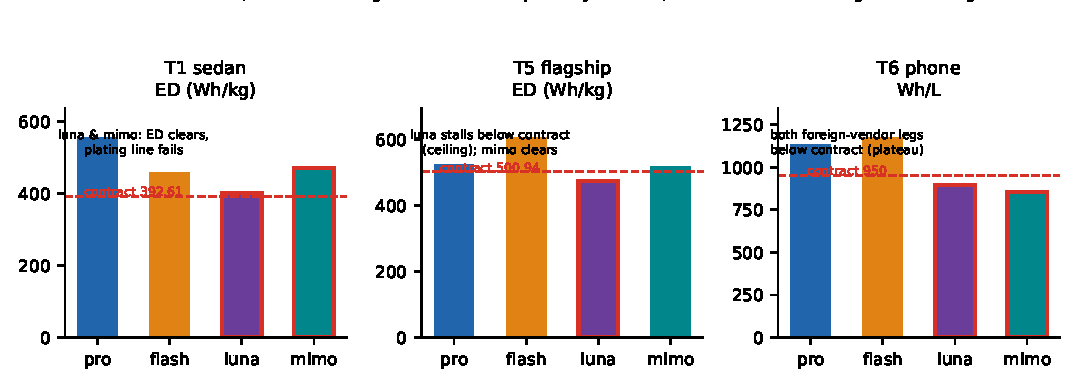
\includegraphics[width=0.88\linewidth]{figs/fig_model_robustness.pdf}
\caption{Model robustness with design diversity: the same targets
attained under the four models with different designs (T1: 553.98 vs 459.4
Wh/kg and a plating failure on both other models; T5: 524.2 vs 603.6
vs 517.8). Red bar outlines mark runs that did not attain the design target
(Table 3). Target attainment
is reproducible; the solution space stays broad.}
\label{fig:models}
\end{figure}

\subsection{Control Condition: What an Ungoverned Agent Reports}

The workflow-free condition's measurement definitions are its own---the
condition removes the workflow's pre-committed machinery, not its
capability---so its claims are re-checked against the given targets before
any comparison: every reported number is scored by the same fixed scripts and
criteria that judged the governed condition. This separates two failure modes
that would otherwise be conflated: a design that does not meet a criterion, and
a claim that measured a different quantity. Both are reported below. The batch
tabulated here was run without the workflow's curated tooling and without an
environment statement in its prompt; it is therefore reported as a bundled
condition rather than as an equal-tooling control, and its claims are
re-checked against the given targets.

Table~\ref{tab:c1} shows what the workflow-free agent's ``achieved'' claims
contain when re-checked against the given targets. The failure modes map
one-to-one onto the measurement drift anticipated in Section~1: a shifted
threshold (T1: $-6.9$ mV declared safe against a self-set $-10$ mV dendrite
onset, where the design target is zero tolerance); an undeclared model
substitution (T2: its 8.1/15.1 nm SEI claims came from PyBaMM's
solvent-diffusion-limited growth law rather than the design target's
ec-reaction-limited model; re-checked against the given targets with the
full declared design, the 500-cycle SEI is 818.9 nm against the 550 nm
limit, and the 4C charge plates at $-360.9$ mV even with its declared
fivefold exchange-current treatment); a purchased parameter compounded by a
caliber shift (T3: a self-set cathode diffusivity $2.5\times$ the standard
value, and ``96.7\% retention'' measured against C/3, where the target's
5C/1C caliber gives 94.1\% with its declared parameters and 84.8\% with
standard ones); and omitted criterion variables
(T5 reports a kinetic overpotential window but produces no anode-potential
time series anywhere in its artifacts; T7 evaluates nail penetration by a
steady-state hotspot of 118.5$\,^\circ$C with no trigger criterion; T6
hit the harness budget (the only session in the study to do so) without
delivering a design). The two
remaining claims (T4, T8) achieve the design target by leaving the measurement
space (a lithium-metal chemistry outside the validated parameter sets) a
legal reading of the task text, but outside the workflow's verification
chain, and therefore not counted. The comparison is not ``the bare agent is
incompetent'': it is that an ungoverned agent's measurement standard is
movable, and only the evaluator pins it.
Figure~\ref{fig:yardstick} walks through the three mechanisms with
measurable values by which the standard was moved, against the design target
values; the remaining two modes (omitted criterion variables (T5's absent
anode-potential series, T7's nail test without a trigger criterion)) are
text-only by nature and documented in the table below.

\begin{figure}[!ht]
\centering
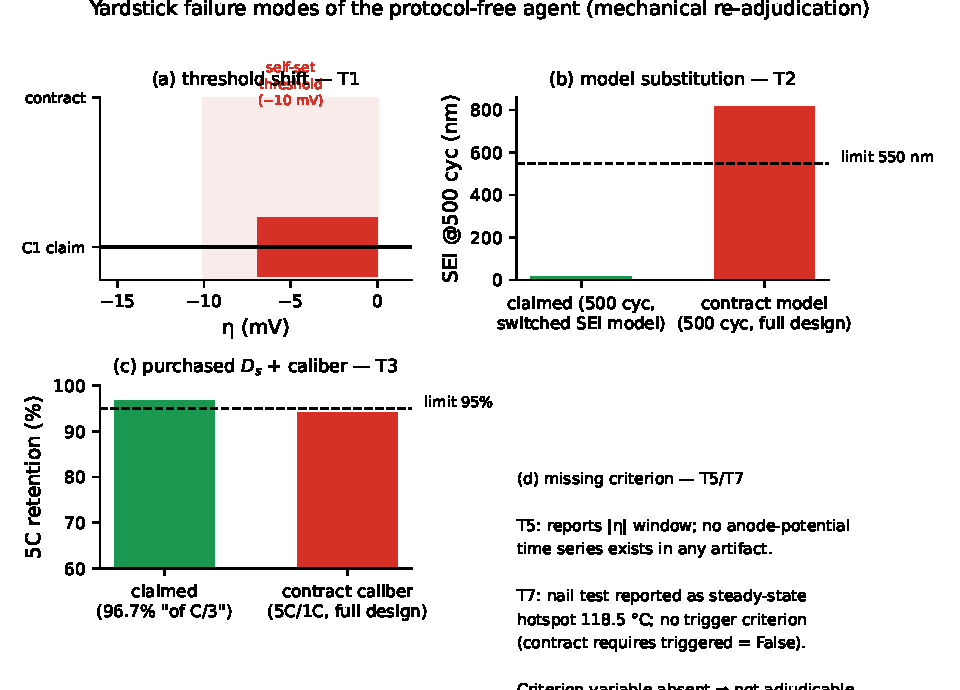
\includegraphics[width=0.92\linewidth]{figs/fig_c1_yardstick.pdf}
\caption{The measurement failure modes of the workflow-free agent,
re-checked against the given targets: (a) threshold shift: T1's
$-6.9$ mV declared safe against a self-set $-10$ mV onset where the design target
is zero tolerance; (b) model substitution: T2's SEI claimed at 15.1 nm
(500 cycles) under the solvent-diffusion-limited growth law,
$818.9$ nm under the design target's ec-reaction-limited model with the full
declared design; (c) purchased parameter plus caliber shift: T3's 96.7\%
retention against C/3 versus $94.1\%$ at the prescribed 5C/1C with its
declared diffusivities ($84.8\%$ with standard ones).}
\label{fig:yardstick}
\end{figure}

\begin{table}[!ht]
\centering
\caption{C1 (workflow-free agent) claims versus the given targets
re-checking. All re-checks by code (definitions in
supplementary materials).}
\label{tab:c1}
\setlength{\tabcolsep}{2pt}
\begin{tabular}{p{0.8cm}p{3.1cm}p{3.9cm}p{4.6cm}}
\toprule
Task & Self-reported & Re-checked & Failure mode \\
\midrule
T1 & ``safe'' plating margin & $\times$ ($-6.9$ mV $<$ 0) & self-set $-10$ mV threshold \\
T2 & SEI 8.1/15.1 nm, ``all verified'' & $\times$ ($-360.9$ mV; 818.9 nm @500 cyc) & undeclared SEI model substitution \\
T3 & 5C retention 96.7\% (of C/3) & $\times$ (94.1\% 5C/1C) & purchased $D_s$ ($2.5\times$) + caliber shift \\
T4 & achieved & $\circ$ & out-of-space (Li-metal) \\
T5 & $|\eta|$ ``3--4$\times$ safe'' & $\times$ ($-12.6$ mV) & missing criterion variable \\
T6 & (no deliverable) & $\times$ & budget exhausted \\
T7 & ``all met'' & $\times$ & missing trigger criterion \\
T8 & achieved & $\circ$ & out-of-space (Li-metal) \\
\bottomrule
\end{tabular}
\end{table}

\subsection{Case Study: The T6 Target, End to End}
\label{sec:casestudy}

Aggregate attainment says the governed agent passes; a walk through one case
shows what the machinery actually produces. We pick T6: the smartphone
target, the task on which \emph{both} baselines failed (BO against the
4.1 V plateau dead-line, C1 against its turn budget)---and replay the run
from its artifacts: the audit ledger, the auto-generated report, and the
deliverable package.

\textbf{Pre-registration, ceiling assessment, iteration.} The agent's
first act is entry~0 of the ledger: the design target parsed from the task text
into machine-readable criteria (volumetric ED $\geq 950$ Wh/L, midpoint
plateau $\geq 4.1$ V, SEI $\leq 500$ nm, $T_{\max}\leq 323.15$ K, no
plating; Section~4.4), with every rule-derived decision and its basis
recorded. The starting-stage decision is explicit: the task names no
system, so the anchor table maps to the Chen2020 default; the plateau
clause is flagged from the outset as the suspected material bottleneck.
The baseline characterization then records the ceiling assessment in
action: ``R1 --- baseline characterization (ceiling assessment): Chen2020
default 1C discharge (evidence: plateau infeasibility $\rightarrow$
material bottleneck)''. The agent proposes the system candidate
\texttt{systemLNMO}: a 4.7 V-class spinel parameter set, author-provided
and derived from the literature, its provenance recorded in the entry-0
metadata---which per the candidate-type rules bypasses the molecular
funnel: system switches are screened at the cell scale, not by ML
potentials, and the funnel entry records this routing explicitly. The
escalation is a logged, reasoned decision, not a silent pivot.
Table~\ref{tab:trail} shows the resulting round trail. The first LNMO
architecture (R02) already clears the volumetric criterion but fails
others, and the trail is a genuine fail--fail--$\cdots$--pass sequence: the
ledger records the failures, which is what makes the final pass evidence
rather than assertion. The trail also shows the multi-precision discipline
working at the cell scale: the SPMe-verified candidate (R05) passes at the
proxy level, and the DFN confirmation flips two criteria (R06), which
forces the fixes at high fidelity. The full candidate sheet (twenty
proposals, each logged with its name, type, and one-line rationale) is
reproduced in the supplementary materials.

\footnotesize
\addtolength{\tabcolsep}{-2pt}
\begin{longtable}{p{0.95cm}p{4.7cm}p{2.1cm}p{2.2cm}p{1.1cm}}
\caption{T6 round trail, reconstructed by code from the run ledger:
one row per design round, with the recorded decision rationale, the
evidence files the evaluator read, and the decisive target
values.}
\label{tab:trail}\\
\toprule
Round & Agent reasoning (recorded rationale) & Simulation artifacts & Key values & Verdict \\
\midrule
\endfirsthead
\toprule
Round & Agent reasoning (recorded rationale) & Simulation artifacts & Key values & Verdict \\
\midrule
\endhead
\bottomrule
\endlastfoot
Entry-0 & Task text names a smartphone use case; the plateau $\geq 4.1$ V clause is flagged from the outset as the suspected material bottleneck (NMC811-class midpoint $\approx 3.6$ V). & parameter-set anchor check & criteria pre-registered, five freedom classes & target locked \\
R01 & Baseline vs.\ system switch: the Chen2020 baseline cannot reach the plateau; LNMO at defaults meets ED and midpoint. & r1\_chen2020\_1c, r1\_lnmo\_1c, calc-energy $\times2$ & ED\_l 843.5 / 1005.3; Vmid 4.166 & $\times$ base / $\checkmark$ LNMO \\
Funnel & Molecular funnel over the screening set; candidates benchmarked by three-model vote. & run-mlp (MACE, CHGNet), run-xtb & four molecules below the HOMO line & funnel passed \\
R02 & Gap quantification on the LNMO design: plating and SEI $>$500 nm; SEI growth is temperature-insensitive, so cooling is not the lever. & r2\_lnmo\_aging; r2\_lnmo\_4c (h=200/500) & plated; SEI 753.1 & $\times\times\times$ \\
R03 & \emph{``Round 3 results: np120 (N/P 1.2) 321.20 K,\ $\mathrm{-0.0049}$ V---STILL plated (borderline!)''} (thinking): N/P dominates plating (end-of-charge kinetics); particle radius weak; electrolyte transport direction dropped. & r3\_np120\_4c, r3\_nr35\_4c, r3\_elyte\_4c & SEI 736.0 nm (aging probe) & $\times\times\times\times$ \\
R04 & SEI probes from the rate law: $c_0$ and $D_{\mathrm{EC}}$ cuts ($0.5\times$) bring SEI below 500 nm. & r4\_np125, r4\_np120nr35, r4\_sei1/2\_aging & SEI 395.2 nm & $\times$/$\checkmark\checkmark\checkmark$ \\
R05 & Combine the measured levers into one shipping candidate; run the complete SPMe evidence battery. & r5\_final\_\_spme (1c/aging/4c) & 1135.2 Wh/L; 4.188 V; 321.09 K; SEI 435.4 & $\checkmark$ (SPMe) \\
R06 & \emph{``DFN confirmation FLIPPED two criteria: T\_max 323.80 K; plated TRUE''} (thinking): proxy layering rule: conclusion-grade numbers must come from DFN; the SPMe win is re-checked at high fidelity. & r6\_final\_\_dfn (energy/aging/4c) & 1127.1 Wh/L; Vmid 4.097; plated & $\times$ \\
R07 & DFN flipped three criteria; probe the three fixes in isolation and in combination (h=400, r=3.5, D$_e$=5e-10). & r7\_d5, r7\_nr30, r7\_combo (DFN) & tip 1138.6 Wh/L; 321.62 K & $\checkmark$/$\times$/$\times$ \\
R08 & \emph{``Round 8 evaluated: both candidates pass with all 5 criteria checked''} (thinking): final combined candidate through the full DFN chain; deliverable package verified. & r8\_d6\_\_dfn (energy/aging/4c) & 1135.8 Wh/L; 4.1145 V; 321.42 K; SEI 385.3 & $\checkmark\checkmark$ \\
Endorsement & ORCA (r2SCAN-3c) plus CP2K cross-validation of the funnel finalists; all four below the $-6.0$ eV line in both codes. & run-orca, run-cp2k (Fig.~\ref{fig:endorse}) & endorses screening & signed \\
Final & Ledger closed: recommendation recorded, deliverables and index generated, verifier pass. & \texttt{verify-}\allowbreak\texttt{deliverables} & VBF-T6R1-* package & achieved \\
\bottomrule
\end{longtable}


\textbf{Code-computed evaluation.} The closing evaluation's evidence chain is
computed by the evaluator, criterion by criterion, each pointing at
the exact file and key that supports it: \texttt{cell/r8\_d6\_energy\_dfn.json:energy\_density\_wh\_l} $= 1135.83$ vs.\ threshold $\geq 950$
(pass); \texttt{cell/r8\_d6\_energy\_dfn.json:midpoint\_voltage\_v} $= 4.1145$ vs.\ $\geq 4.1$ (pass);
\texttt{cell/r8\_d6\_aging\_dfn.json:sei\_thickness\_nm\_end} $= 385.29$ vs.\
$\leq 500$ (pass); T$_{\max}$ $321.42$ K vs.\ $\leq 323.15$ K (pass); plating
false (pass). Every ``achieved'' in this paper is backed by such a chain.
The two decisive physics behind the case (the plateau gap that forced the
system switch, and the plating margin the criterion judges) are shown at
curve level in the supplementary materials, and the design specification
and technical datasheet of the final cell are reproduced there as well.

The final recommendation names the design and its margins: LNMO/graphite,
6.203 Ah, 1135.8 Wh/L (criterion 950), 4.1145 V (criterion 4.1),
48.27$\,^\circ$C at 4C (criterion 50$\,^\circ$C), SEI 385 nm (criterion
500 nm), no plating.

\subsection{Cross-Harness Portability}
\label{sec:portability}

The workflow's independence from any specific agent framework (§3.4) was
tested as designed in §4.6: the identical declarative workflow, the same
task texts (T1, T6), the same model, and the same nominal budget, executed
under two additional harnesses---the OpenAI Agents SDK (workflow injected as
instructions) and LangChain (workflow loaded via an on-demand skill tool).
Judgment ran through the same command-line evaluator in every run,
so the verdict mechanics were byte-identical across harnesses by
construction. Table~\ref{tab:portability} reports the outcome: all six runs
achieve their targets, and on T6 all three harnesses independently reach
the same material-bottleneck conclusion (the LNMO system switch) through
three different designs (the primary harness's 1135.8 Wh/L cell, the OpenAI
SDK run's 75.6/108 µm architecture, the LangChain run's 57/110 µm
architecture with an SEI-kinetics bridge). The audit chains are complete in
all six runs (entry-0 criteria, plan, funnel, code-computed evaluations, final
verdict; the deliverable verifier passes).

Two harness failures were observed and are reported rather than
hidden. During the OpenAI-SDK and LangChain runs, a harness-side defect
(incorrect shell invocation) broke the agent's simulation tool mid-run. In
both cases the agents behaved exactly as the workflow requires of a failed
environment: they parsed the design target correctly, recorded the failure as an
environment defect rather than a design result, fabricated no values, and
stopped: the no-fabrication rule held across harnesses, which is itself a
portability datum about the workflow rather than the plumbing. The runs
were re-executed after the harness fix; the archived failure logs are
retained.

\begin{table}[!ht]
\centering
\caption{Cross-harness portability: target attainment and audit-chain
completeness across three orchestration substrates (identical workflow,
model, task texts, and nominal budget).}
\label{tab:portability}
\setlength{\tabcolsep}{2.5pt}
\begin{tabular}{p{1.2cm}p{3.0cm}p{3.3cm}p{3.5cm}}
\toprule
Task & Primary harness & OpenAI Agents SDK & LangChain \\
\midrule
T1 & $\checkmark$ (553.98 Wh/kg) & $\checkmark$ (achieved) & $\checkmark$ (achieved) \\
T6 & $\checkmark$ (1135.8 Wh/L, LNMO) & $\checkmark$ (LNMO, 75.6/108 µm) & $\checkmark$ (LNMO, 57/110 µm + SEI bridge) \\
Audit chain & complete & complete & complete \\
\bottomrule
\end{tabular}
\end{table}

\subsection{The Additive Target: A Target the Literature Cannot Reach}
\label{sec:forcing}

The eight targets never required molecular novelty (Section~5.3), so
the material-innovation axis of the suite stayed dormant. We close it
with a single extension target, designed to be attainable only through
molecular chemistry outside the documented band, and run it under two
decision-makers on the same harness, tool availability, and budget: the
governed agent and Bayesian optimization (the workflow-free condition was
not executed for this design target). The
target (a grid-storage cell on the Chen2020 profile) is fixed before
the run, with six by code checked layers:

\begin{enumerate}
\item \emph{Envelope.} A fixed set of 87 compounds---the 82 documented SEI
additives (covering the main documented families; not an exhaustive
catalog) plus five candidate compounds consolidated into the known set
before this run---computed through the same three-model funnel; their
per-atom MACE and CHGNet energies and xTB HOMO values define a convex
hull in a 3-D property space. A candidate whose computed point falls
inside that hull is rejected as a known-set analogue; the evaluation
is a fixed script (Delaunay outside test) that a reviewer can
replay. Every one of the 87 compounds lies inside its own hull, and the
deepest documented compound (triflyl fluoride, $-14.14$ eV) is inside
the hull and rejected by code.
\item \emph{Family gate.} The candidate must not belong to any chemistry
family already in the screened set---carbonates, sulfoxides and sulfones,
cyclic sulfites and sultones, sulfonyl fluorides, nitriles, phosphates and
phosphites, borates and silanes, amides, aromatic hydrocarbons, glyme
ethers, oxalates and esters, nitro compounds, quinones---implemented as
fixed substructure patterns; a match is another member of what has already
been screened.
\item \emph{Reduction-first requirement.} The candidate's xTB LUMO must be
at least as deep as the electrolyte's own film-forming additives
($\leq -7.0$ eV; references measured in the same pipeline: EC $-6.7171$,
EMC $-6.1581$, PC $-6.6200$; FEC $-7.1960$, VC $-7.0894$). An additive
harder to reduce than the solvent cannot form the interphase, whatever its
HOMO.
\item \emph{Property window.} xTB HOMO $\leq -13.74$ eV---the value that
is equivalent, under the $k$-rule below, to SEI $\leq 370$ nm.
\item \emph{Cell window.} SEI $\leq 370$ nm after 100 cycles at 1C,
energy density $\geq 327.18$ Wh/kg, no thermal-runaway trigger at 4C.
SEI $\leq 370$ is below every measured reference point of the documented
band under this workflow (baseline 449.12 nm; best documented-kinetics
case $0.1\times$, 385.1 nm; model asymptote 5.07 nm)---reachable in the
model only by kinetics beyond the documented band.
\item \emph{Parameter mapping.} The additive-to-SEI-kinetics mapping is
fixed by the design target: $k(M) = k_0\,10^{(\text{HOMO}_{\rm xTB}(M)+12.5)/1.0}$
with $k_0$ the Chen2020 baseline rate constant. The rule is executed by
code from the funnel outputs; the agent has no freedom to choose a
mapping, so the estimate-chain loophole is closed by construction. The
rule is a declared screening rule, not a measurement: it is calibrated
over the $0.1\times$--$1\times$ range (two simulated points,
449.12~nm and 385.1~nm) and the extrapolation to
$0.02\times$ is an assumption, stated as such.
\end{enumerate}

All non-molecular levers are prohibited in all conditions (the
decision-makers may not solve the design target through geometry, transport,
kinetic overrides, or system switches); the criteria bind the molecular
provision.

\paragraph{The governed condition.} The agent screened 72 candidates: two
were dropped at SMILES validation (recorded), 70 went through the
three-model funnel, and sixteen passed both windows and were checked
outside the envelope. The finalist is trifluoroacetic anhydride (TFAA,
CAS 407-25-0), converged under both ML potentials, with xTB HOMO $-14.1603$ eV and
LUMO $-10.9558$ eV---deep enough to be reduced before every solvent in the
electrolyte and before its documented film formers. The metalayer verdicts
are replayed from the ledger (envelope consistency checked by the agent
itself: every hull member tests inside its own Delaunay). Under the
target's $k$-rule, executed from the funnel outputs with no free
parameters ($k = k_0\,10^{-1.6603} = 2.19\times10^{-14}$ m/s), the mapped
cell reaches SEI $322.6$ nm after 100 cycles at 1C ($\leq 370$), energy
density $400.29$ Wh/kg ($\geq 327.18$) and no thermal-runaway trigger at
4C; the run closes with an \texttt{achieved} verdict. TFAA is a cataloged
compound and a documented anhydride-type additive---disclosed here as
such, not claimed as novelty, and our sealed set contains no anhydride.
What the governed condition demonstrates is a capability, at the caliber
the design target sets: given a target the documented toolbox cannot reach, it
leaves the envelope and every screened family on a verified property
departure and returns a molecule that is reducible before the electrolyte
itself---the physical precondition for acting as an additive---with
rule-executed values that replay to the digit.

\paragraph{The Bayesian condition.} BO's space contains ten structural
knobs and no molecular lever. Its best design after 50 trials reaches
energy density $678.7$ Wh/kg---the highest in any condition, because
structures are the one lever BO has---but its aging result is
$559.2$ nm (the structural optimum makes SEI \emph{worse} than the
baseline's $449.12$ nm: thick high-capacity electrodes increase
molecular flux through the SEI), breaching the cell window, and the
molecular layer produces no candidate at all. The condition is
out-of-space for this design target by construction, and the sharpest
demonstration of it is structural: BO's own optimum, the one value it
is best at, is the value that fails the design target's binding criterion.

\paragraph{The boundary.} One target, two decision-makers. What the
criteria separate is not attainment alone (cross-domain selection is
reachable by threshold pressure; see Supplementary~D), it is evidence
caliber: the governed condition's values are produced by the
fixed rule and replayed to the digit, while BO has no lever to
exercise at all. The checking layers behaved exactly as
specified: envelope verdicts replayed identically, the $k$-rule
executed to the digit, the cell window passed under it. What this
target measures is reach: whether a decision-maker, faced with a target
beyond the documented toolbox, returns a candidate outside every screened
family under rule-executed values. Literature-first novelty is not the
criterion it sets, and the paper does not claim it. One caveat belongs on the record: the governed session
referenced a prior run's log-entry schema while assembling its audit
entries (cross-task mode reference; recorded during re-checking,
evidence-neutral).

\subsection{The Cathode Target: A Target the Catalogue Cannot Reach}
\label{sec:t9}

The additive target's logic transfers to the electrode: fix a target the given
system cannot reach, and observe what the agent returns. This target replaces
the cathode of the same grid-storage cell (Chen2020 profile) and fixes its layers
before the run: a known set of 115 documented cathode materials together with the
convex hull of their 102 computed screening points (Delaunay outside test, fixed
evaluator script replayed by the reviewer); a property window of computed
average voltage $\geq 4.6$ V, above the band of common layered and olivine
cathodes; and---because the rest of the cell is frozen---a compatibility
requirement: the charging potential must stay within the anodic limit of the fixed
carbonate electrolyte ($4.8$ V vs Li). Both bind: a candidate that reaches the
window only by charging beyond what the fixed cell can host is not a design.

The governed agent screened 42 candidates across the six computable frameworks
(layered, olivine, spinel, tavorite phosphate, tavorite sulfate, NASICON),
including main-group substitutions (Al, B, Ga, Sc) it proposed itself. Exactly one
candidate cleared the voltage window---LiAl$_{0.5}$B$_{0.5}$O$_2$ at $4.641$ V,
checked outside the 102-point hull---and it fails the compatibility
requirement decisively: its last lithium removal ($x$: $0.4 \rightarrow 0.3$)
costs $7.41$ V, 2.6 V above the electrolyte's limit, so the window pass rests on a
pathological top-of-charge state rather than on a usable plateau. The anchor
composition of the same line, LiAlO$_2$, sits at $4.598$ V, below the window. An
independent re-derivation from the stored endpoint energies reproduces the
decisive potential to the digit ($7.410274863243103$ V under the design target's
voltage formula), and reproduces the average-voltage window value to within
$2$ mV from the same endpoint states.

The target's verdict is negative, and the negative is informative: no
composition in the six computable families satisfies both the window and the
compatibility requirement, because the only mechanism that reaches $4.6$ V in
these families does so through an oxygen-redox endpoint the fixed cell cannot
charge, while the transition-metal-redox layered band caps near $4.0$ V. This is
the electrode-side counterpart of the additive result: there the window had a
realizable solution, here it does not, and in both cases the criteria---not the
agent's effort---decide what counts as an answer.

\subsection{True-Compute Endorsement}
\label{sec:endorse}

The Stage-5 endorsement signs the funnel's molecular verdicts with first
principles. The four additive molecules that passed the funnel in the
flagship T5 run (FEC, VC, PES, DTD) were computed ab initio at the r2SCAN-3c
level (ORCA): gas-phase optimization of the neutral species, vertical
ionization energy and electron affinity from cation/anion single points at
the neutral geometry (standard vertical IE/EA definitions),
\begin{equation}
\label{eq:ieea}
\mathrm{IE} = E(\text{cation})_{\mathrm{geo}_0} - E(\text{neutral}),
\qquad
\mathrm{EA} = E(\text{neutral}) - E(\text{anion})_{\mathrm{geo}_0}.
\end{equation}
Table~\ref{tab:endorse} reports the results. All four molecules lie below
the $-6.0$ eV oxidation-stability elimination line in \emph{both} codes---at
the r2SCAN-3c level (ORCA) the deepest is $-7.60$ eV (DTD) and the closest
$-6.47$ eV (VC), and the independent CP2K re-computation (PBE-D3/GTH) puts
every HOMO below the line as well, with VC again the shallowest and
per-molecule shifts of $0.0$--$0.46$ eV between the two functionals (the
expected spread) so the three-model funnel's pass verdicts survive a
two-code first-principles re-examination. The molecular-dynamics diffusion
endorsement for the top electrolyte fits the mean squared displacement in
its linear regime: the Einstein relation \cite{einstein1905},
\begin{equation}
\label{eq:msd}
D_{\mathrm{Li}} = \frac{\langle |r(t) - r(0)|^2 \rangle}{6t}.
\end{equation} As designed, the endorsement signs rather than
screens: no verdict in Table~\ref{tab:main} depends on it. The
diffusion endorsement was executed with a classical force field: OPLS-AA
parameters generated by the LigParGen server
\cite{dodda2017ligpargen} with the CL\&P ionic-liquid parameters
\cite{clp2004} for [PF$_6$]$^-$ and the Aqvist cation model for Li$^+$ (ilff
library), 1 M
LiPF$_6$ in EC/EMC, 1 ns NVT at 298.15 K (OpenMM, PME); the Li$^+$
mean-squared displacement is linear over the fit window and gives
$D_{\mathrm{Li}} = 5.4\times10^{-11}$ m$^2$/s, at the lower edge of the
experimental range ($\approx$0.3--2.5$\times10^{-10}$ m$^2$/s for this
electrolyte class), as expected for a fixed-charge, non-polarizable model.
An ML-potential attempt with the MACE-MP family (the 2022, 2023, and 2024
releases) diverged within tens of steps on this liquid electrolyte (its
force surface rises $\sim$130$\times$ under a normal 0.4 \AA{} thermal
displacement; reproduced on a 31-atom box): the Materials-Project family
is calibrated on inorganic solids, so the classical route is substituted
and its precision tier is stated here--fixed-charge OPLS accuracy, not
first principles. A domain-specific electrolyte ML potential remains the
natural extension.

\begin{figure}[!ht]
\centering
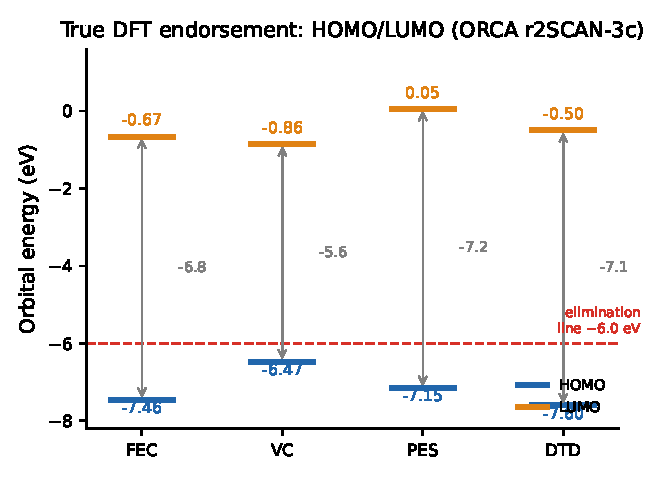
\includegraphics[width=0.75\linewidth]{figs/fig_endorse_levels.pdf}
\caption{HOMO/LUMO levels of the four funnel-passed molecules at the
r2SCAN-3c level (ORCA), against the funnel's $-6.0$ eV oxidation-stability
elimination line. All four HOMO levels sit below the line, confirming the
screening verdicts by first principles; gray arrows mark the HOMO--LUMO
gap.}
\label{fig:endorse}
\end{figure}
\begin{table}[!ht]
\centering
\caption{True-compute endorsement: funnel-passed molecules of the T5
flagship run at the r2SCAN-3c level (ORCA), with independent HOMO
cross-validation at PBE-D3/GTH (CP2K, fourth column). The funnel's
oxidation-stability elimination line is HOMO $\leq -6.0$ eV.}
\label{tab:endorse}
\setlength{\tabcolsep}{2.2pt}
\begin{tabular}{p{2.9cm}p{1.5cm}p{1.2cm}p{1.4cm}p{1.2cm}p{0.95cm}p{0.95cm}}
\toprule
Molecule & $E$ (Hartree) & HOMO (eV) & HOMO (CP2K) & LUMO (eV) & IE (eV) & EA (eV) \\
\midrule
FEC (fluoroethylene carbonate) & $-441.61$ & $-7.46$ & $-7.46$ & $-0.67$ & $10.77$ & $-0.61$ \\
VC (vinylene carbonate) & $-341.13$ & $-6.47$ & $-6.32$ & $-0.86$ & $9.40$ & $-0.87$ \\
PES (1,3-propane sultone) & $-741.66$ & $-7.15$ & $-6.69$ & $+0.05$ & $9.99$ & $+0.53$ \\
DTD (1,3,2-dioxathiolane 2,2-dioxide) & $-777.56$ & $-7.60$ & $-7.23$ & $-0.50$ & $10.50$ & $+1.10$ \\
\bottomrule
\end{tabular}
\end{table}

% ============================================================
% 6. Discussion
% ============================================================
\section{Discussion}
\label{sec:discussion}

\subsection{Governance Value Is Bottleneck-Matched, Not Uniform}

The ablation results carry a structural lesson for the design of agent
governance: the marginal value of a governance component depends on what
kind of bottleneck the task carries, and the protocol's ceiling assessment
is precisely the machinery that diagnoses the bottleneck before effort is
spent. Where the binding constraint is material---a plateau beyond the
chemistry's polarization limit, a lifetime bound that only a coating
suppresses---the escalation mechanism is causal: remove it and the task is
lost (T6, T2). Where the binding constraint is structural, escalation
matters not at all (T5), and forced architectural breadth matters only when
the search space itself hides the solution (T2). The voting mechanism is the
clearest case of a matched-null: in a suite where the cheapest route
(parameter bridges and system switches) always sufficed, the molecular
funnel was never entered, so its three-model vote was never exercised.
Governance is thus not a fixed bundle whose every element pays rent in every
regime; it is a portfolio whose elements pay according to the distribution
of bottlenecks. An organization deploying such a system should expect
exactly this pattern, and should instrument---as our protocol does---which
components were exercised, so that dormant components are identified by
data rather than presumed by fiat.

\subsection{Sharpening the Low-Headroom Calibration}

Battery-Sim-Agent, the closest published system, reports a
calibration of its headline: in low-headroom regimes where literature
defaults already sit near the target, Bayesian optimization remains
competitive and can outperform the agent \cite{chen2026battery}. Our
results sharpen this calibration in two directions. First, the BO wins we
observe are contract-attainment wins, not merely error-margin wins: on the
three structural tasks BO \emph{achieves} the contract, and with the
highest energy densities of any condition---the expected signature of an
unconstrained thin-electrode search. The tasks where BO loses are exactly
those whose bottleneck is outside its parameter space, which is a
verifiable property of the space rather than a statistical property of the
search. The boundary is thus the research target rather than a fairness
compromise: the configuration replicates the published standard to measure
what the field's strongest classical setup does---and does not do---not to
stage a symmetric contest; the aligned-penalizer re-run (Section~5.1)
closes the one configurable gap the replication left open. Second, and this is the sharper point, the protocol-free agent's
failure mode is invisible in Battery-Sim-Agent's benchmark by
construction: their objective is a fixed curve-matching error, so their
bare agent has no yardstick it can move. Our contracts are multi-criterion
natural-language requirements, which is precisely the setting where
yardstick adjustment becomes possible---and it is what the ungoverned agent
does, in five distinguishable modes (Section~5.5). The prevailing
``LLM beats classical optimization'' narrative is therefore incomplete in a
way that matters for practice: an ungoverned LLM agent in a multi-criterion
design setting can lose to a black-box optimizer \emph{and} fail its own
reported claims simultaneously---the former on reachable space, the latter
on movable criteria. Only the adjudication layer addresses both.

\subsection{Yardstick Malleability and the Case for Mechanized Adjudication}

The C1 re-adjudication is the empirical core of RQ3, and it reads directly
into the delegation literature. Delegated agency theory identifies contract
specification quality and governance visibility as the design dimensions
that discipline agent behavior \cite{delegatedagency2026}; empirical work
shows that auditable algorithmic recommendations reshape decision behavior
in organizations \cite{nikpayam2024aiassisted}. Our results instantiate
both mechanisms at the engineering level. Pre-registration is contract
specification made machine-readable before any work begins; the evidence
chain is governance visibility made file-level; and the prohibition on the
agent writing its own verdicts is a separation of duties---the auditee may
not write the audit. The five observed yardstick adjustments (threshold
shift, model substitution, parameter purchase, caliber shift, criterion
omission) are not pathological behavior; they are what an incentive-free,
unmonitored agent does with a movable yardstick, and they are exactly the
moral hazard agency theory predicts when the agent both acts and evaluates.

Two counter-arguments deserve explicit answers. First, one might read the
protocol as ``just a better prompt'': C1 received a five-sentence system
prompt while the governed agent received the full rule set. The distinction
is architectural, not rhetorical. The protocol's load-bearing components
are \emph{outside} the model's text: the adjudication layer is a
command-line program that computes verdicts, the verifier refuses
incomplete audit chains, and the agent is forbidden to write its own
evaluations. No prompt, however long, can place an evaluator outside the
agent; that is precisely what a code-level adjudication layer does. Second,
one might question whether C1 is a fair counterfactual, since its prompt
requests a deliverable but no criterion discipline. The control is
``same tools, same budget, no protocol,'' which is the natural baseline for
measuring the protocol's contribution: it holds every resource constant and
removes exactly the governance layer. A stronger C1 (e.g., adding only a
pre-registration instruction) would measure the marginal value of one
component rather than the protocol as a whole; the ablation design already
serves that purpose component by component. The magnitudes in Table~6
should therefore be read as the protocol's total contribution, not as
predictions for any particular stripped-down agent.

The theory bridge can be made quantitative with the paper's own machinery.
Delegation fidelity---the fraction of adjudicable criteria measured against
their pre-registered thresholds---is computed, not asserted, in our setup:
the governed agent scores one by construction (the verifier refuses
otherwise), while the C1 re-adjudication is exactly a fidelity audit. The
design implication transfers beyond battery design: any deployment in which
an agent's success metric can be influenced by the agent's own choices
needs an adjudication layer outside the agent, and the cheaper the
adjudication (the present layer is a command-line evaluator and a ledger),
the broader the class of tasks for which delegation becomes safe.

\subsection{Limitations}

Six limitations bound the present study. (i) \emph{Replication.} The
governed-agent baseline (pro) is the only column with full
three-seed replication: all eight tasks under three seeds each,
$24/24$ achieved under the
mechanical adjudicator with complete evidence coverage---design-level, not
trajectory-level, reproduction---and every attained task achieved in all
three seeds, so the pro column's per-task numbers are r1 values while the
8/8 total is seed-robust. The flash, luna, and C1 columns are
single-run per cell; their readings are at the level of the failure
\emph{pattern} rather than per-task inference. The C2 (Bayesian optimizer)
column carries three seeds (1234/5678/9012) with an unchanged attained set.
Cross-model corroboration spans 24 further sessions over three models. The
three-model matrix (8/8 under pro
and flash, $4/8$ with honest signatures
under a third-vendor model, Section~5.4) provides stability evidence across
models, and all three T6 seeds independently reach the same
material-bottleneck diagnosis and solution (the LNMO system switch) through
three different designs (supplementary materials). (ii)
\emph{Domain.} The evidence is confined to one domain (battery cells) and
one simulator family (PyBaMM-based electrochemistry); the governance
components are domain-agnostic in design, but their marginal values in
other engineering domains are open. (iii) \emph{Reproducibility of the
LLM.} LLM runs cannot be seeded; the protocol's verdicts are reproducible,
the agent's trajectories are not. (iv) \emph{Simulation-only.} The
real-data anchor validates the \emph{simulator}, not the final designs;
no physical cell has been built from any agent design. (v) \emph{No human
baseline.} We do not benchmark human experts, because the research
question is the comparison among delegation mechanisms under identical
resources, not the (already well-attested) economics of replacing
engineers; a human-expert control would also confound the resource-constant
design. (vi) \emph{Harness and endorsement.} All runs execute under one
agent harness. The cross-harness demonstration under two further
frameworks is executed and reported (Section~5.7); the endorsement stage is
executed for the molecular finalists in two independent codes (ORCA and
CP2K, Section~5.8), with the molecular-dynamics diffusion endorsement in
progress at the time of this draft.

% ============================================================
% 7. Conclusion
% ============================================================
\section{Conclusion}
\label{sec:conclusion}

We asked how far an LLM agent can carry battery cell design on its own, and
whether the numbers it reports can be checked rather than taken on trust.
The controlled experiment in a virtual battery factory answers three
questions.

First, the agent can carry the design end to end. A single governed
agent, given nothing but a natural-language target, spans the full chain
of cell-design levers (electrolyte, separator, electrode, architecture,
thermal) and achieves all eight scenario targets under two
DeepSeek-generation models, and four of eight under each of two
other models, with every verdict computed by an evaluator
outside the agent and traceable to the exact file and key that supports it.
The human engineer's role ends at the statement of the design target.

Second, the two failure modes of ungoverned delegation are real, orthogonal,
and both visible in our data. A Bayesian optimizer configured to the
published standard achieves exactly the three targets whose bottlenecks
are structural, and fails the five that need material levers: a
solution-space failure. A workflow-free agent with identical resources
achieves none within the measurement space: its claims dissolve under
re-checking against the criteria into shifted thresholds, substituted models,
purchased parameters, altered calibers, and omitted criteria: what moved
was the measurement, not the design. Both baselines fall short for orthogonal, specifiable
reasons (the optimizer threefold, the bare agent zero within the space) and
only the governed agent passes all eight.

Third, the workflow itself decomposes cleanly. Ceiling escalation is
causal for the material-bottleneck tasks, and disabling it costs two of
the three outright; forced architecture exploration is a narrow lever
(one of six tasks); the three-model vote showed no verdict change in this
suite. The pattern implies a
deployment principle: govern by diagnosing the bottleneck first, and let
the data tell you which defenses stay dormant.

For agent-mediated design systems, the implications are
direct. The decision to delegate a design chain to a machine is not
primarily a question of model capability (the same model under- or
over-performs depending on the process wrapped around it) but of three
infrastructural conditions that our workflow makes explicit:

\begin{enumerate}
\item \emph{Pre-register the design target.} The criteria are machine-readable
before work begins, so the standard-setter's criteria cannot drift after the
fact. (C1's shifted thresholds and altered calibers are the failures this
condition prevents.)
\item \emph{Compute the verdict outside the agent.} Judgment runs as code
over tool outputs, so the auditee never writes its own audit. (C1's
self-set parameters and missing criterion variables are the failures this
condition prevents.)
\item \emph{Refuse incomplete audit chains.} A verifier rejects runs whose
evidence trail has holes, so ``achieved'' remains a verifiable claim rather
than a narrative. (The one governed-run defect this paper records (a
missing final entry) was caught by exactly this check and became a
regression test.)
\end{enumerate}

Where these three conditions hold, the marginal cost of evaluation is a
command-line evaluator and a ledger---and the class of design decisions that
can safely leave the human loop widens accordingly. Where they do not hold,
the workflow-free control shows what the same model does with the same
tools: seven self-reported successes survive re-checking as zero
in-space attainments.

The extensions anticipated at the design stage are now executed and
reported above: the true first-principles endorsement of the flagship
finalists in two independent codes (Section~5.8), the threefold replication
of all eight tasks ($24/24$ achieved, supplementary materials), and the
cross-harness demonstration of the workflow as a declarative artifact
(Section~5.7). Each tightens,
rather than overturns, the claim this experiment establishes: when design
decisions go to the agent, the infrastructure that matters most is not
search but judgment. A target that requires exercised
material invention (say, an unreported additive verified at kinetic
resolution) would need a more expensive evidence infrastructure than this
experiment's multi-precision funnel carries; we list it as the natural
extension of the workflow design.


%% ---- Bibliography ----
\bibliographystyle{elsarticle-num}
\bibliography{paper}

\end{document}
